\documentclass[a4paper,12pt,oneside]{report}
%\usepackage[Glenn]{fncychap}
\usepackage[Lenny]{fncychap}
\usepackage[utf8]{inputenc}
\usepackage[T1]{fontenc}
\usepackage{float}


%%% Escolha das fontes
% Charter
%\usepackage[charter]{mathdesign}

%%% Combo: Palatino + Helvetica + Courier, com EulerVM para matemática
\usepackage{mathpazo}
\usepackage[scaled=.95]{helvet}
\usepackage{courier}
\linespread{1.05} %%% Palatino needs more spacing.

%%% Idem, mas pxfonts para matemática
%\usepackage{pxfonts}
%\usepackage[scaled=.95]{helvet}
%\usepackage{courier}
%\linespread{1.05} %%% Palatino needs more spacing.

% Outras fontes
%\usepackage{bookman} % Obsoleto, usar Kerkis
%\usepackage{kmath,kerkis}
%\usepackage[urw-garamond]{mathdesign}
%\usepackage[utopia]{mathdesign}
%\usepackage{mathptmx} % Isso se eu quisesse usar com Times!
%\usepackage{mathrsfs}
%\usepackage{eulervm} % Euler iria bem, mas não nesta tese...
%\usepackage{libertine} % Fonte da Wikipedia!

%
% Geometria da página. Sugiro manter estas mesmas margens e 15 cm de espaço de texto.
\usepackage[a4paper,pdftex,top=2.8cm,bottom=4cm,left=3.4cm,right=2.6cm]{geometry}
\textwidth=15.0 true cm

%
% Table of Contents
\setcounter{tocdepth}{2}

\usepackage{sprace}
\usepackage[]{units}
%
% Use isto pros headers


\usepackage{fancyhdr}
\setlength{\headheight}{15.2pt}
\pagestyle{fancy}

% % tenemos que apagar dedsde aqui para cambiar el formato de capitulo  

%\renewcommand{\chaptermark}[1]{%
%\markboth{\chaptername\ \thechapter.\ #1}{}}

%% E menos espaço ao começar o capítulo
%\usepackage{titlesec}
%\titleformat{\chapter}[display]
%  {\normalfont\rmfamily\huge\mdseries}
%  {\chaptertitlename\ \thechapter}{20pt}{\huge}
%\titlespacing*{\chapter}{0pt}{-20pt}{40pt}

% %  hasta aqui


% Linha Extra
\newcommand{\linha}{\enlargethispage{1\baselineskip}}

% Páginas bonitas
\fancypagestyle{plain}{%
\fancyhf{} % clear all header and footer fields
\fancyfoot[C]{\textit \thepage} % except the center
\renewcommand{\headrulewidth}{0pt}
\renewcommand{\footrulewidth}{0pt}}

\fancypagestyle{fancyplain}{%
\fancyhf{}
\fancyhead[L]{\textit{\leftmark}}
\fancyhead[R]{\textit{\thepage}}
%\fancyfoot[C]{\today} % Use este fancyfoot pros drafts (data no pé da página)!
\fancyfoot[C]{} % Use este fancyfoot (vazio) pra versão final!
\renewcommand{\headrulewidth}{0.6pt}
\renewcommand{\footrulewidth}{0pt}}

%%%%%%%
% Do the hypersetup
%%%%%%%

\hypersetup{pdftitle={Search for a Heavy Resonance in the MET + Jet Final state},
            pdfauthor={David Romero Abad},
            pdfsubject={High Energy Physics},
            pdfkeywords={High Energy Physics}
            			{Particle Physics}
            			{Hadron Colliders} 
				{Extra Dimensions}
				{Beyond the Standard Model},
			colorlinks=true,
			citecolor=blue,
			linkcolor=blue			
            }

\begin{document}

%%% This makes all the frontmatter stuff, sans the Table of Contents.
\pagestyle{plain}

%\input Preambulo.tex
\input TitlePage.tex



%\input blanco.tex

\pagenumbering{roman}

\input abstract.tex

%\input blanco2.tex

%%% The Table of Contents and a new page
\tableofcontents
\newpage

%%%
%%% Ok, ready to start. Reset headings and page numbers.
%%%

\pagenumbering{arabic}



\input Introduction.tex


\chapter{Theoretical Framework}


\section{Standard Model of Fundamental Interactions}

This chapter present a brief description of the Standard Model of Fundamental Interactions (SM), indicating their origins, particle content, interactions and  lagrangians of different sectors.\\
\indent
The electroweak theory of the SM was proposed by Glashow, Weinberg and Salam \cite{Glashow:1961tr, Salam, PhysRevLett.19.1264} to describe the electromagnetic and weak interactions of quarks and leptons, which is based on the local gauge group  $SU(2)_{L}\otimes U(1)_{Y}$.
Combined with quantum chromodynamics (QCD), which is the theory of strong interactions between quarks and gluons, with local gauge group $SU(3)_{C}$, the model foresees a unified framework to detail these three forces of nature.\\
\indent
It is necessary to make a differentiation between different types of fundamental particles involved in the SM. The particles are divided into: bosons (particles of integer spin), responsible for transmitting the fundamental forces of the nature, and fermions (particles of half-integer spin) that are the constituents of matter. Since not all fermions have the same properties, they have been divided into two types: leptons and quarks. One of the differences is that quarks have fractional electric charge while the charge of the leptons are multiples of the electron charge. The quarks exhibit a very peculiar property called "confinement", which means that free quarks have not been observed. Quarks feel all interactions, but leptons are not affected by the strong force.\\
\indent
In particle physics, a generation is a division of elementary particles. Between generations, particles differ only in their mass. All interactions and quantum numbers are identical. There are three generations according to SM of particle physics. Each member of an higher generation has bigger mass than the corresponding particle of the previous generation. This hierarchy of mass causes particles to decay from high to low generations, which explains why ordinary matter (atoms) is made of particles of the first generation. Every atom is then composed of first generation particles. The second and third generations of charged particles do not form normal matter and are only seen in extremely high-energy environments. The table below  summarizes the main properties of fermions:

\begin{table}[h]
\footnotesize
\begin{center}
\begin{tabular}{|c|c|c|c|}\hline\hline
\multicolumn{4}{|c|}{\bfseries Fermions}\\ \hline\hline
  \textbf{Generation} & \ \textbf{Fermions} &  \textbf{Mass [MeV]}  &  \textbf{Charge} ($Q/\left|e\right|$) \\ \hline
  &u & $2.3$ & $2/3$   \\ \cline{2-4}
  & d & $4.8$ & $-1/3$ \\\cline{2-4} 
\raisebox{1.5ex}[0pt]{$1^{a}$}   &e & $0.511$ & $-1$   \\ \cline{2-4}
  & $\nu_{e}$ & $ < 2 \times 10^{-6}$ & $0$  \\ \hline
 &c & $1.275\times 10^{3}$ & $2/3$ \\ \cline{2-4} 
  &s & $95$ & $-1/3$ \\ \cline{2-4}
\raisebox{1.5ex}[0pt]{$2^{a}$} &$\mu$ & $105.66$ & $-1$ \\ \cline{2-4}
  & $\nu_{\mu}$ & $<  0.19$ & $0$ \\ \hline
&t & $173.21\times 10^{3}$ & $2/3$ \\ \cline{2-4}  
  &b & $4.18\times 10^{3}$ & $-1/3$ \\ \cline{2-4}
\raisebox{1.5ex}[0pt]{$3^{a}$} &$\tau$ & $1777$ & $-1$ \\ \cline{2-4}
 & $\nu_{\tau}$ & $< 18.2$ & $0$  \\ \hline\hline
\end{tabular}
\caption{Fermions Generations}\label{tab3} 
\end{center}
\end{table}

Unlike leptons, quarks are confined within hadrons, and they are not seen as physical particles. The masses of the quarks can not be measured directly, but can be determined indirectly through their influence on hadronic properties.\\
\indent
The different interactions are described in the quantum language in terms of bosons exchange between the constituents fermions.

\begin{table}[h]
%\centering
\resizebox{0.85\textwidth}{!}{\begin{minipage}{\textwidth}
\renewcommand{\arraystretch}{1.3}
\begin{tabular}{|c|c|c|c|c|}
\hline
\multicolumn{5}{|c|}{\textbf{Types of Interactions}}   \\ 
\hline
 Interaction & Gauge Group & Boson & Symbol & Relative Magnitude \\ 
\hline
Strong  & $SU(3)$ & gluons (8 types)  & $g$  & 1   \\ 
\hline
Electromagnetic  & $U(1)$  & photon  & $\gamma$  & $10^{-2}$  \\ 
\hline
Weak  & $SU(2)$  & intermediate vector bosons  & $W^{\pm}$, $Z^{0}$  & $10^{-7}$  \\ 
\hline
Gravitational  & ?  & Graviton (hypothetical)  & $G$  & $10^{-39}$  \\
\hline 
\end{tabular} 
\end{minipage}}
\caption{Fundamental Interactions \label{table:interactions} }
\end{table}

As the \cref{table:interactions} shows, there are four types of fundamental interactions.
The strong interactions are responsible to bind the quarks inside the proton and the neutron, while maintaining the neutron and the proton in the nucleus. The force between quarks is mediated by massless particles called gluons.
Electromagnetism is responsible for binding electrons in the atom, the atoms in the molecules, and intermolecular forces in liquids and solids. These interactions are mediated by the exchange of photons.
Weak interactions are typified by $\beta$ nuclear decay processes, which involves the emission of an electron and a neutrino by a radioactive nucleus.
The mediators of the weak force are bosons $W^{\pm}$ and $Z^{0}$, with masses of the order of
100 times the proton mass. Gravitational interactions act on all types of particles. 
As can seen from the \cref{table:interactions}, the relative magnitude of the gravitational interaction is very small, thus, for practical purposes it is not considered within the SM.

\begin{figure}[h]
  \centering
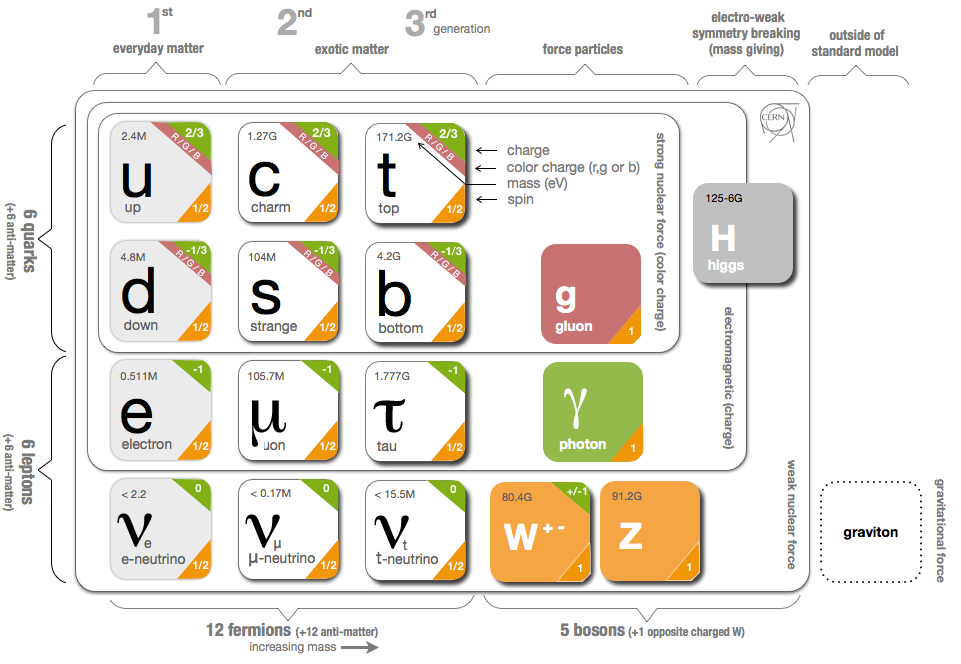
\includegraphics[width=12cm]{SM_chapter_plots/SM}
\label{SMfigure}\caption{Particles of the Standard Model}
\end{figure}

\subsection{Electroweak Interaction}

The SM propose a doublet representation for the left-handed fields and singlets for the right-handed fields:
\begin{eqnarray}
L^{i}=\left(
\begin{array}{c}
\displaystyle \nu_{e L}\\
\displaystyle e_{L}
\end{array}\right),
\left(
\begin{array}{c}
\displaystyle \nu_{\mu L}\\
\displaystyle \mu_{L}
\end{array}\right),
\left(
\begin{array}{c}
\displaystyle \nu_{\tau L}\\
\displaystyle \tau_{L}
\end{array}\right),
\qquad
Q^{i}=\left(
\begin{array}{c}
\displaystyle u_{L}\\
\displaystyle d_{L}
\end{array}\right),
\left(
\begin{array}{c}
\displaystyle c_{L}\\
\displaystyle s_{L}
\end{array}\right),
\left(
\begin{array}{c}
\displaystyle t_{L}\\
\displaystyle b_{L}
\end{array}\right).        
\end{eqnarray}
\begin{eqnarray}
e_{R}^{i} &=& \left\lbrace e_{R}, \mu_{R}, \tau_{R} \right\rbrace ,  \nonumber\\
u_{R}^{i} &=& \left\lbrace u_{R}, c_{R}, t_{R} \right\rbrace , \qquad d_{R}^{i} = \left\lbrace d_{R}, s_{R}, b_{R} \right\rbrace .
\end{eqnarray}
Where $i$ runs over the generations of fermions. The $L$ (left-handed) and $R$ (right-handed) indices appears because the projections operators were applied over the wave functions, where $\psi_{L}=P_{L}\psi$ and $\psi_{R}=P_{R}\psi$, with $P_{L}=(1-\gamma^{5})/2$ and $P_{R}=(1+\gamma^{5})/2$.\\
The free massless fermionic lagrangian is:
\begin{displaymath} 
\lagrangean_{f}=\frac{i}{2}\sum^{3}_{i=1}\left\{\:\bar{L}^{i}\:\not\! \partial\:L^{i}+\:  \bar{Q}^{i}\:\not\! \partial\:Q^{i}+\:\bar{e}_{R}^{i}\:\not\! \partial\:e_{R}^{i} + \:\bar{u}_{R}^{i}\:\not\! \partial\:u_{R}^{i} + \:\bar{d}_{R}^{i}\:\not\! \partial\:d_{R}^{i}  \right\}+\hbox{h.c}
\end{displaymath}
with $\bar{\psi}=\psi^{\dag}\:\gamma^{0}$.\\
The proposed Lagrangian must be invariant under local gauge transformations:
\begin{eqnarray}
\Psi_{i}\:'&=&\:\hbox{exp}\left[i\:\alpha(x)_{j}\sigma_{j}+i\:\beta(x)Y\right]\Psi_{i}\nonumber\\
\chi_{i}\:'&=&\:\hbox{exp}\left[i\:\beta(x)Y\right]\:\chi_{i}  
\end{eqnarray}
where $\Psi_{i}=\left\{L^{i},Q^{i}\right\}$ and $\chi_{i}=\left\{e_{R}^{i}, u_{R}^{i}, d_{R}^{i} \right\}$. Also, 
 $\alpha$ and $\beta$ are parameters belonging to the symmetry groups $SU(2)$ and $U(1)$ respectively, $\sigma_{j}$ are the Pauli matrices and $Y$ is the hypercharge.
In order to mantain the gauge invariance after the transformations, we have to introduce the covariant derivatives:
\begin{eqnarray}
D_{L}^{\:\mu}&=&\;\partial^{\mu}-\:i\:\left(g/2\right)\:\sigma_{j}\:A^{\mu}_{j}+\:ig'\:B^{\:\mu}\:Y\;\nonumber\\
D_{R}^{\:\mu}\:&=&\;\partial^{\mu}+\:i\:g'\:B^{\:\mu}\:Y\;\:
\end{eqnarray}
Finally we get:
\begin{eqnarray}\label{leptonico}
\lagrangean_{f}=\frac{i}{2}\sum^{3}_{i=1}\left\{\:\bar{L}^{i}\:\not\!\! D_{L}\:L^{i}+\:\bar{Q}^{i}\:\not\!\! D_{L}\:Q^{i}+\:  \bar{e}_{R}^{i}\:\not\!\! D_{R}\:e_{R}^{i}+\:  \bar{u}_{R}^{i}\:\not\!\! D_{R}\:u_{R}^{i}+\:  \bar{d}_{R}^{i}\:\not\!\! D_{R}\:d_{R}^{i}\right\}+\hbox{h.c}\nonumber\\
\end{eqnarray}
where $\not\!\! D\equiv \displaystyle\gamma_{\mu}D^{\:\mu}$ and $g'$, $g$ are the coupling constants of the groups $U(1)$ and $SU(2)$ respectively. $A^{\mu}$, $B^{\mu}$ are gauge fields.\\
\indent
So far we have presented the Lagrangian of fermions and their interactions with the gauge fields via the covariant derivative. The complete Lagrangian density of SM should also contain terms that describe the gauge bosons when there is no fermions involve (free bosonic Lagrangian).
These expressions should also be locally gauge invariants under $SU(2)_{L}\otimes U(1)_{Y}$. Similarly in the case of fermions we assume, for the moment,  massless gauge bosons. The bosonic lagrangian is:
\begin{eqnarray}\label{bosott}
\lagrangean_{B}=\frac{1}{2g^{2}}\:\hbox{Tr} \left(\mathcal{F}_{\mu\nu}\:\mathcal{F}^{\mu\nu}\right)-\frac{1}{4}B_{\mu\nu}\:B^{\mu\nu}
\end{eqnarray}
\begin{flushleft}
where the fields are expressed as function of the group generators
\begin{eqnarray*}
\mathcal{ F}_{\mu\nu}(x)=-\frac{ig}{2}\sigma_{a}F^{a}_{\mu\nu}(x),\ \ \ \ \  A_{\mu}(x)=-\frac{ig}{2}\sigma_{a}A^{a}_{\mu}(x)
\end{eqnarray*}
resulting:
\begin{eqnarray}
\lagrangean_{B}&=&-\frac{1}{4}\sum^{3}_{a=1}F^{a}_{\mu\nu}F^{\mu\nu a}-\frac{1}{4}B_{\mu\nu}B^{\mu\nu}
\end{eqnarray}
To maintain the local gauge invariance of the Lagrangian, it follows that:
\end{flushleft}
\begin{eqnarray}
F^{a}_{\mu\nu}&=&\partial_{\mu}A^{a}_{\nu}-\partial_{\nu}A^{a}_{\mu}+g\:\epsilon^{a}_{bc}\:A^{b}_{\mu} A^{c}_{\nu},\ \ \ \ \ \ \ \ \ a=\hbox{1,2,3.}\nonumber\\
B_{\mu\nu}&=&\partial_{\mu}B_{\nu}-\partial_{\nu}B_{\mu}
\end{eqnarray}
The Lagrangian (\ref{bosott}) involves gauge fields connected with the groups $SU(2)_{L}$ and $U(1)_{Y}$ and, the number of fields is related to the number of group generators. In our case we have four gauge fields $A^{1}$, $A^{2}$, $A^{3}$ and $B$.\\

\subsection{Strong Interaction}

The Strong interaction between quarks and gluons in the SM, is described by the Quantum Chromodynamics (QCD). The QCD is a non-abelian gauge field theory based on the  symmetry group $SU(3)_{C}$.
The Lagrangian of QCD, invariant under $SU(3)_{C}$ gauge transformations, is given by:
\begin{eqnarray}
\lagrangean_{S}&=&\sum_{q}\:\bar{\psi}_{q,a}\left( i\not\!\! D -m_{q} \right)\psi_{q,a} - \dfrac{1}{4}\:G^{A}_{\mu\nu}G^{A \mu\nu} 
\end{eqnarray}
The $\psi_{q,a}$ are quark-field spinors for a quark flavor $q$ and mass $m_{q}$, with a color index $a$ that runs from $a=1$ to $N_{C}=3$. In order to maintain gauge invariant, the covariant derivative take the form:
\begin{eqnarray}
D_{\mu} = \partial_{\mu} + ig_{S}\dfrac{\lambda_{A}}{2}\mathcal{A}_{\mu}^{A} 
\end{eqnarray}  
where $g_{S}$ is the QCD coupling constant, $\lambda_{A}$ the Gell-Mann matrices and $\mathcal{A}_{\mu}^{A}$ the gauge field of the gluons where $A$ runs from $A=1,\dots,8$. The field tensor $G^{A}_{\mu\nu}$ is given by:
\begin{eqnarray}\label{gluon}
G^{A}_{\mu\nu}&=&\partial_{\mu}\mathcal{A}^{A}_{\nu}-\partial_{\nu}\mathcal{A}^{A}_{\mu}+g_{S}\:f_{ABC}\:\mathcal{A}^{B}_{\mu} \mathcal{A}^{C}_{\nu},\ \ \ \ \ \
\left[ \lambda_{A}, \lambda_{B} \right] = 2if_{ABC}\lambda_{C}
\end{eqnarray}
where $f_{ABC}$ are the structure constants of the $SU(3)$ group.

\subsection{Spontaneous Symmetry Breaking}\label{QES}

Until now all the fermions and gauge bosons were considered massless, but in reality for all particles proposed in the SM only
the photons are massless. The simple addition of the mass terms to the Lagrangian density spoils the gauge invariance and the renormalization of the theory.\\
\indent
In order to maintain the theory renormalizable it is essential to introduce the masses by a mechanism that keeps the gauge invariance
of the Lagrangian density, this is achieved through the Higgs mechanism \cite{Higgs:1966ev}.\\
\indent
This mechanism uses the spontaneous symmetry breaking  (SSB), initially proposed by  by Goldstone, Salam and Weinberg \cite{PhysRev.127.965}, which states that under a certain symmetry transformation, the Lagrangian remains invariant, but not so the vacuum state. If the symmetry is global, a massless particle appears which is called the Nambu-Goldstone boson \cite{PhysRevLett.4.380,Goldstone:1961eq}.\\
\indent
When this method is applied in a local gauge theory, something amazing happens: the Nambu-Goldstone bosons are absorbed by gauge particles and turn massless particles on massive ones. This is called Higgs-Kibble mechanism \cite{Higgs:1966ev,PhysRev.155.1554}.
Now we construct a local gauge invariant Lagrangian for
zero spin particles, consisting of a free or kinetic part and a potential. By introducing the covariant derivative in the kinetic term, we ensure their gauge invariance.
Then we have:
\begin{eqnarray}
\lagrangean_{H}=\left[D^{\mu}\Phi\right]^{\dagger}\left[D_{\mu}\Phi\right]+\mu^{2}\Phi^{\dagger}\Phi-\lambda^{2}\left[\Phi^{\dagger}\Phi\right]^{2}
\end{eqnarray}
where $\Phi$ is a scalar complex field  which transform as a $SU(2)_{L}$ doublet :
\begin{eqnarray}
\Phi=\left(\begin{array}{c}
\phi^{+}\\
\phi^{0}
\end{array}\right)
\end{eqnarray}
To meet gauge invariance: 
\begin{eqnarray}
D_{\mu}\:=\left[\;\partial_{\mu}-\:\frac{i\:g}{2}\:\sigma_{j}\:A^{j}_{\mu}+\:\frac{ig'}{2}Y\:B_{\mu}\;\right]\:\nonumber
\end{eqnarray}
In a similar way, $g$ y $g'$ are the coupling constants, $\sigma_{j}$ and $Y$ are the generators, and $B_{u}$ and $A^{j}_{\mu}$ are the gauge fields of the groups $U(1)_{Y}$ and $SU(2)_{L}$ respectively.\\
The SSB implies that the Higgs field expand over the vacuum.
\begin{eqnarray}
\Phi=\frac{1}{\sqrt{2}}\left(\begin{array}{c}
0\\
v+h(x)
\end{array}\right)
\end{eqnarray}
where $v$  is the vacuum expectation value and $h$ is the Higgs field.

\subsection{Yukawa Lagrangian}

In the previous section the Higgs field was introduced in order to generate mass for the SM particles. The gauge bosons couples with the scalar field through the covariant derivative, but in the case of fermions, they not show 
any link with the scalar field. For that reason, we need to
introduce a new Lagrangian (by hand) in which the Higgs field engages with the fermions: 
\begin{equation}\label{yukawa}
\lagrangean_{Y}=-\sum_{\lepton=1}^{3} G_{\lepton}\left[\bar{L}^{\lepton}\Phi\:e^{\lepton}_{R}\:\right]- \sum_{i,j=1}^{3}\left[\:\Gamma^{u}_{ij}\:\bar{Q}^{i}\:\tilde{\Phi}\:u^{j}_{R} + \Gamma^{d}_{ij}\:\bar{Q}^{i}\:\Phi\: d^{j}_{R}  \right]  
+\hbox{h.c.} 
\end{equation}
with
\begin{equation}
\tilde{\Phi} \equiv i\tau^{2}\Phi^{\dag}=\left(\begin{array}{c}
\phi^{0 \dag}\\
-\phi^{-}
\end{array}\right) 
\end{equation}
where the index runs over the number of generations, and the $\Gamma^{u},\Gamma^{d}$ are 3x3 matrices which determine the fermion masses and mixings.
This lagrangian is know as Yukawa Lagrangian.\\
After the SSB we obtain the complete Lagrangian density of the SM, in the unitary gauge:
\begin{eqnarray}
\lagrangean &=& \bar{\psi}_{f}\left(i \:\not\! \partial-m_{f} \right)\psi_{f}\nonumber\\
&-&\dfrac{1}{4}F_{\mu\nu}F^{\mu\nu}-\dfrac{1}{4}G^{A}_{\mu\nu}G^{A \mu\nu}\nonumber\\
&-&\dfrac{1}{2}F^{\dag}_{W \mu\nu}F^{\mu\nu}_{W} + m_{W}^{2}W^{\dag}_{\mu}W^{\mu}\nonumber\\
&-&\dfrac{1}{2}Z_{\mu\nu}Z^{\mu\nu} +\dfrac{1}{2}m_{Z}^{2}Z_{\mu}Z^{\mu}\nonumber\\
&+& \dfrac{1}{2} \left(\partial_{\mu} h \right)\left(\partial^{\mu} h \right)- \dfrac{1}{2} m_{H}^{2}h^{2} + \text{interaction terms}   
\end{eqnarray}
where :
\begin{eqnarray}
F^{\mu\nu} &=& \partial^{\nu}A^{\mu}-\partial^{\mu}A^{\nu} \nonumber\\
F^{\mu\nu}_{W} &=& \partial^{\nu}W^{\mu}-\partial^{\mu}W^{\nu} \nonumber\\
Z^{\mu\nu} &=& \partial^{\nu}Z^{\mu}-\partial^{\mu}Z^{\nu}
\end{eqnarray}
are the fields related with the photon, W boson and Z boson respectively. The field $\psi_{f}$ runs over all the fermions and   $G^{A}_{\mu\nu}$ is the gluon field previously defined in (\ref{gluon}). The mass terms are given by:
\begin{eqnarray}
m_{\lepton} &=& \dfrac{G_{\lepton} v}{\sqrt{2}}\\
m_{W} &=& \dfrac{1}{2} vg\\
m_{Z} &=& \dfrac{1}{2} v\sqrt{g^{2}+g'^{2}}\\
m_{H} &=& \sqrt{ 2 v^{2} \lambda}
\end{eqnarray}



\section{Beyond Standard Model}

Although the Standard Model accurately describes the fundamental interations in nature and agrees with all the experimental data we have at our disposal today it is still incomplete. Perhaps it is only a part of a bigger picture that includes new physics. Some of the unanswered main questions are:  Why is the weak scale so much smaller than the Planck scale?  What is the origin of the difference between matter and antimatter, and is it related to the origin of the matter in the Universe? What is the nature of the astrophysical dark matter? How does one unify the fundamental interactions?\\
\indent
In this section we will give a little insight into some of these problems and some models which try to give an answer.

\subsection{The Hierarchy Problem}\label{hierarchy}

When radiative corrections are performed to the Higgs mass, for example at one loop level (\cref{figurehiggsmass}), one needs to integrate over  the momentum of the virtual particles. In general we have to limit the integral by a cut-off ($\Lambda$) related with  the next energy scale in the theory.
If the next scale is gravity, $\Lambda$ is the Planck scale $M_{P} \sim 10^{18}$ \gev. Thus, if the SM were valid up to the Planck scale, then the Higgs mass $m_{H}$,	and therefore the minimum of the Higgs potential $v$ , would be driven from the weak scale to the Planck scale by the radiative corrections (eqn. \ref{higgsmasseq}).
\begin{figure}[H]
  \centering
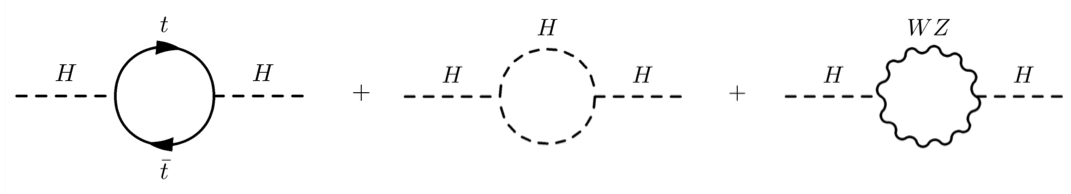
\includegraphics[width=15cm]{SM_chapter_plots/higgsmass}
\caption{Radiative Corrections to the Higgs Mass. \label{figurehiggsmass}}
\end{figure}
\begin{eqnarray}\label{higgsmasseq}
m_{H}^{2} = m_{H,0}^{2} + \dfrac{3 g^{2}}{32 \pi^{2}}\dfrac{\Lambda^{2}}{m_{W}^{2}}\left[ m_{H}^{2} + 2m_{W}^{2} + m_{Z}^{2} - \dfrac{4}{3} m_{t}^{2}  \right] 
\end{eqnarray}
To avoid this, one
has to adjust the Higgs bare mass $m_{H,0}$ to one
part in $10^{17}$. This is quite unnatural, and is what we call the
gauge \textbf{hierarchy problem}.
In order to solve this unnatural fine tunning some theories beyond SM were proposed, for example, Supersymmetry (SUSY), Composite Higgs and Extra Dimensions. We will focus only in the last of these models.

\subsection{Dark Matter}

Dark matter is a hypothetical kind of matter that cannot be seen with telescopes but accounts for most of the matter in the universe. Dark matter neither emits nor absorbs light or any other electromagnetic radiation at any significant level. This means that it has not electric charge and can interact only via gravitational force, or weak force similar to neutrinos.
The existence and properties of dark matter are inferred from many sources,
\paragraph{Velocity curves of spinning galaxies} In 1970 an American astronomer, Vera Rubin, measured the speed of stars in rotating galaxies accurately enough to convince the scientific community. She observed that stars in spinning galaxies were all rotating at roughly the same velocity, no matter their distance to the galactic centre. This is in contradiction with Kepler’s law that describes the rotation of planets around the Sun.  This could only happen if huge amounts of invisible matter filled the entire galaxy and beyond.
\paragraph{Gravitational lensing} We know that light moves in a straight line in free space. In the presence of a massive object such as a star or a galaxy, the space is deformed and light follows the curvature of the distorted space. Light coming from a distant galaxy will bend when passing near a massive clump of dark matter and the galaxy will appear shifted, as if coming from different places.
\paragraph{Cosmic microwave background} Astrophysicists can infer how much dark matter exists by studying the cosmic microwave background. From the amount of radiation associated to each frequency, astrophysicists can calculate the quantity of dark matter contained in the Universe.\\

\indent Experiments at the (LHC) may supply more direct evidence about dark matter. According to many theories, dark matter particles would be light enough to be produced at the LHC. If they were generated at the LHC, they would escape through the detectors leaving no signal. However, they would transport energy and momentum, so one could infer their existence from the amount of energy and momentum "missing" after a collision. Dark matter candidates arise frequently in theories that suggest physics beyond the Standard Model, such as Supersymmetry and Extra Dimensions.

\subsection{Extra Dimensions}

Why is gravity so much weaker than the other fundamental forces?  One possibility is that we don’t feel the full effect of gravity  because part of it spreads to extra dimensions. If extra dimensions exist, they could explain why gravity is weaker than the other forces of nature.

How could we test for extra dimensions? 
Some theorists suggest that a particle called the "graviton" is associated with gravity. If gravitons exist, it should be possible to create them at the LHC, but they would rapidly disappear into extra dimensions. A graviton might escape our detectors, leaving an empty zone that we notice as an imbalance in momentum and energy in the event. We would need to carefully study the properties of the missing object to work out whether it is a graviton escaping to another dimension or something else. This method of searching for missing energy in events is also used to look for dark matter or supersymmetric particles.

	

\subsubsection{Large Extra Dimensions}

The reason why we have not observed the extra dimensions yet is that contrary to the ordinary four space-time dimensions which are very large (or infinite), these hypothetical extra dimensions are finite, that is they are compactified. The  question that one needs to ask is how large could the size of the extra dimensions be without getting into conflict with observations.\\
\indent 
Assuming that there are $n$ extra dimensions, calling the fundamental Planck scale of the theory (in $4+n$ dimension) $M_{*}$, the usual Planck scale (in 4 dimensions) $M_{Pl}$, $r$ the compactification radius of the extra dimension, and using the matching for the gravitational and the gauge coupling, it is found that \cite{Csaki:2004ay}:
\begin{eqnarray}
M_{Pl}^{2} &=& M_{*}^{n+2}V_{(n)}= M_{*}^{n+2}\left(2 \pi r \right)^{n} \sim r^{n}M_{*}^{n+2}\label{planck}\\ 
\dfrac{1}{g_{4}^{2}} &=& V_{(n)}M_{*}^{n} \sim r^{n}M_{*}^{n}
\end{eqnarray}
In the second equation we assume that the gauge field propagates in all dimensions. Considering that the spacetime is flat, and that the $n$ extra dimensions are compact, where $V_{n}$ is the volume of the extra dimensional space and $g_{4}$ is the coupling constant. From these two equations it is obtainned:
\begin{eqnarray}
r \sim \dfrac{1}{M_{Pl}}\:g_{4}^{\frac{n+2}{n}}
\end{eqnarray}
This would imply that in a higher dimensional theory $r \sim 1/M_{Pl}$. In this case there would be no hope of finding these tiny extra dimensions. Now, we will investigate what happen if, instead of the previous assumption, the SM fields were localized in 4 dimensions, and only gravity were to propagate into the extra dimension. 
In that case new phenomena will appear in the gravitational sector when you reach distances as short as the size of the extra dimension. However, it is very hard to test gravity at very short distances. The bound in the size of the extra dimension ($r\leq$ \unit[0.1]{mm}) is given by Cavendish type experiments if only gravity propagates in the extra dimension.\\ 
\indent
For $M_{*}\sim$ \unit[1]{TeV} the model is called "Large Extra Dimensions", proposed by Arkani-Hamed, Dimopoulos and Dvali (ADD) \cite{ArkaniHamed:1998rs}.
From (eqn. \ref{planck}) we find:
\begin{eqnarray}
r \sim 2\times 10^{17}\times 10^{\frac{32}{n}} \text{cm}
\end{eqnarray}
Therefore, if we select $n=1$ , we get that $r\sim 10^{8}$ Km, which is certainly excluded. Taking $n=2$ , one has $r \sim 1$ mm, which is a distance scale already constrained by Cavendish-type experiments.\\
\indent
The fact that gravity propagates in compact extra dimensions leads to the existence of graviton excitations with a mass gap given by $\Delta m \sim 1/R$.
The graviton in this $(4+n)$-dimensional formulation can be equivalently expressed as a set of 3-dimensional Kaluza–Klein (KK) modes  with different graviton masses. The coupling of the KK modes to the SM energy–momentum tensor leads to an effective theory with virtual-graviton exchange at leading order (LO) in perturbation theory. An ultraviolet (UV) cutoff must be introduced to avoid divergences in the summed contributions from all modes.


\subsubsection{Universal Extra Dimensions}

Universal Extra Dimensions \cite{PhysRevD.64.035002} are models in which all of the SM fields live in $4+n$ dimensions with the $n$ extra dimensions taken to be flat and compact. 
In the Minimal Universal Extra Dimensions (MUED) we have five dimensions, namely only one extra dimension. In this model the hierarchy problem is not addressed but have some interesting features as a stable dark matter candidate.
In this case the extra dimension is compactified in a circle of radius $r$. 
The key element is the conservation of momentum in the universal dimensions. In the equivalent four-dimensional theory this implies KK number conservation. For example, in five dimensions (5D), $p_{5}$ the fifth component of the 5D momentum is quantified and given by
\begin{eqnarray}
p_{5} = n/r
\end{eqnarray}
Promoting the full SM to extra dimensions bring some problems, for example the fermions are generically non-chiral (with respect to our four dimensions). This problem is solved by "orbifolding", \ie, compactifying on surfaces with endpoints. In five dimensions, the only choice is $S^{1}/Z_{2}$, which identifies opposite sides of a circle to create a line segment with two endpoints.

\begin{figure}[H]
  \centering
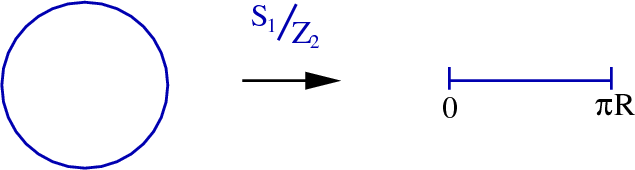
\includegraphics[width=12cm]{SM_chapter_plots/orbifold}
\label{orbifigure}\caption{orbifold}
\end{figure}

As a consequence of the orbifolding, translational invariance along the 5th dimension is broken, which results that the KK-number conservation is broken too, but there is a remnant left: the parity
of the KK modes must be conserved at	 the vertex. In addition, KK-parity conservation means that the lightest state of
the first KK level cannot decay into zero-modes, making it
stable and a candidate for dark matter.
The masses of the KK modes at tree levl are given by:
\begin{eqnarray}
m_{n}^{2} = \dfrac{n^{2}}{r^{2}}+ m_{SM}^{2}
\end{eqnarray}
with $n=0,1,2,\dots$. Note that for $n=0$ (zero mode) we obtain the mass on the SM particles. In general the mass of the SM particles are smaller than the compactification radius of the extra dimension, so the KK modes are practically degenerate. Radiative corrections generate mass splittings, but these are still
small enough for the energy yield to be small in the production and subsequent decay of KK states.

\subsubsection{Warped Extra Dimension}

\paragraph{Randall Sundrum (RS) Models}

Lisa Randall and Raman Sundrum proposed a model where there is only one warped extra dimension which is compactified on the $S^{1}/Z_{2}$ orbifold \cite{Randall:1999ee,Randall:1999vf}. Two 4D branes (the Planck brane and the TeV brane) are separated by the fifth extra dimension with size $r_{c}$ (fig. \ref{RSfigure}). Even though the extra dimension is curved, the brane itself remains static and flat, that is, it preserves 4D Lorentz invariance. This means that the induced metric at every point along the extra dimension has to be the ordinary flat 4D Minkowski metric, and the components of the 5D metric depend only on the fifth coordinate $y$. The ansatz for the most general metric satisfying these properties is given by:
\begin{eqnarray}
ds^{2}= e^{-A(y)} dx^{\mu}dx^{\nu} \eta_{\mu\nu} - dy^{2} 
\end{eqnarray}
Where $\eta_{\mu\nu}=\text{diag}(-1,1,1,1)$ and the amount of curvature (warping) along the extra dimension depends on the function $e^{-A(y)}$, which is therefore called the warp-factor. This
type of geometry is called "non-factorizable" because the metric of the 4D subspace is $y$-dependent.
In the simplest version of the RS model it is assumed that the SM fields live on the so-called TeV brane while gravity lives everywhere. Unlike the ADD case, however, there is a "cosmological" constant in the 5D bulk and both branes have distinct tensions. Solving the 5D Einstein’s equations provides a unique solution for these quantities and also determines that $A(y) = k\left| y \right| $, where k is a dimensionful parameter. A basic assumption of this model is that there are no large mass hierarchies present, so that we expect that $k \sim M_{*}$, the 5D fundamental or Planck scale. In fact, once we solve Einstein’s equations and plug the solutions back into the original action and integrate over $y$ we find that:
\begin{eqnarray}
M_{Pl}^{2} = \dfrac{M_{*}^{3}}{k}\left(1-e^{-2\pi k r_{c}} \right)  
\end{eqnarray}
The warp factor $e^{-\pi k r_{c}}$ will be a very small quantity which implies that $M_{Pl}$, $M_{*}$ and $k$ have essentially comparable magnitudes following from the assumption that no hierarchies exist. If we calculate the Ricci
curvature invariant for this 5D space, we find that it is  constant, $ R_{5} = - 20 k^{2}$ and thus $k$ is a measure of the
constant curvature of this space. A space with constant negative curvature is called an Anti-DeSitter space and so this 5D version is called $AdS_{5}$.
\begin{figure}[H]
  \centering
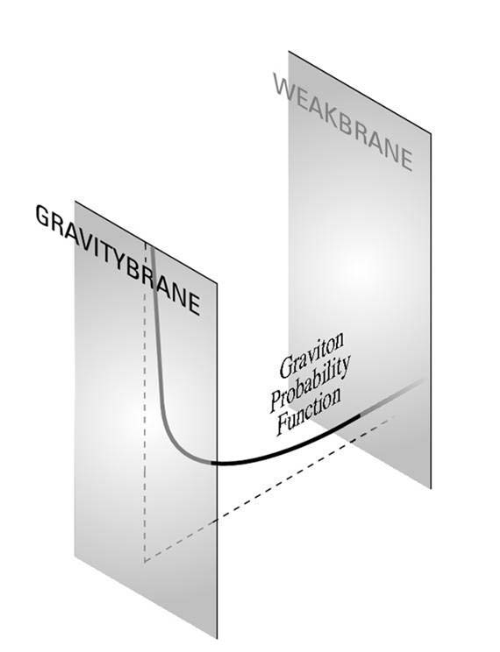
\includegraphics[width=6cm]{SM_chapter_plots/RS}
\caption{Graviton probability function \label{RSfigure}}
\end{figure}

It will be assumed that all dimensionful parameters in the action will have their mass scale set by $M_{*} \sim M_{Pl} \sim k$ so that there is no fine-tuning. However, the warp factor rescales them as one moves about in $y$ so that, in particular, all masses will appear to be of order the
TeV scale on the SM brane. This means that if there is some mass parameter, $m$, in the action which is order $M_{Pl}$, we on TeV brane will measure it to be reduced by the warp factor, i.e., $me^{-\pi k r_{c}}$. Note that if $kr_{c} \sim 11$ (a
small hierarchy) this exponential suppression reduces a mass of order $10^{18}$ GeV to only 1 TeV. Thus the ratio of the weak scale to $M_{Pl}$ is explained through an exponential factor and no large ratios appear anywhere else in the model. It has been shown by Goldberger and Wise \cite{Goldberger:1999un} that values of $kr_{c} \sim 11$ are indeed natural and can be provided by a stable configuration. Hence we have obtained a true solution to the hierarchy problem.
If we consider the action for the Higgs field on the TeV brane:
\begin{eqnarray}
S = \int d^{4}x dy \sqrt{-g} \left(g^{\mu\nu}\partial_{\mu}H^{\dag}\partial_{\nu}H-\left(H^{2}-v_{0}^{2} \right)^{2}\right)\delta\left(y-\pi r_{c} \right)     
\end{eqnarray}
From this we see that the vev that we observe on the SM brane is not $v_{0}$ but
\begin{eqnarray}
v = v_{0} e^{ -\pi k r_{c}}
\end{eqnarray}
which is of order the TeV scale.
Even though gravitons are spin-2, it turns out that their masses
and wave functions are identical to the case of a scalar field in the RS bulk which is far simpler to analyze. If we solve the Klein-Gordon equation, but now in the case of curved space, after a separation of variables via the KK decomposition the solutions are linear combination of $J_{2}$, $Y_{2}$ Bessel functions and the mass of the KK states are given by: 
\begin{eqnarray}
m_{n} = x_{n} k e ^{-\pi r_{c}}
\end{eqnarray}
where $x_{n}$ are roots of $J_{1}(x_{n})=0$. Here $x_{n} = 0, 3.8317, 7.0155, 10.173, \dots$ etc. Since $k e^{-\pi k r_{c}}$ is of the order of a few hundred GeV at most, we see that the KK graviton masses are of similar magnitude with comparable, but unequal, spacing, i.e., the KK gravitons have approximately weak/TeV scale masses. We thus have weak scale graviton KKs with weak scale couplings that should be produced as spin-2 resonances at colliders.

\paragraph{Bulk Graviton Model}

Different models with warped extra dimensions allow the SM fields to propagate in the ED. In these models, as a consequence of the localization of SM particles near the Planck or the TeV brane, decays to diphotons and dileptons are suppressed by a factor proportional to the volume of the extra dimension. This scenario is more compatible with electroweak precision tests and limits on flavor-changing neutral current processes than the original RS1. The different couplings of the graviton to the SM fields result in two distinctive effects: the branching fraction to SM vector-boson pairs can become dominant for certain values of the model parameters, and a very strong enhancement in the longitudinal polarization of the vector bosons is predicted. Because of the aforementioned suppression of photon and fermion couplings, the total production cross section is also smaller with respect to RS1 gravitons: in the Agashe–Davoudiasl–Perez–Soni (ADPS) model \cite{Agashe:2007zd} for $M = 700$ GeV and $\tilde{k}= 0.50$ , it amounts to 0.31 pb in pp collisions at $\sqrt{s} = 7$ TeV, and the branching fraction to longitudinally polarized ZZ bosons is about 12$\%$.






\chapter{CMS Experiment}

\section{Large Hadron Collider (LHC)}

The Large Hadron Collider is the largest and most powerful particle accelerator ever built. It boost protons, to produce two beams travelling in opposite directions, which collide at four points where the two rings of the machine intersect.\\
\indent
The design energy per proton beam is of 7 TeV. The protons of the LHC circulate around the ring in well defined
bunches. In the LHC, under nominal operating conditions, each proton beam has 2808 bunches, with each bunch containing about 10$^{11}$ protons. They measure a few centimetres long and a millimetre wide when they are far from a collision point. As they approach the
collision points, they are squeezed to about 16 $\mu$m to allow for a greater chance of proton-proton collisions. The LHC uses a bunch spacing of 25 ns (or about 7 m), which  corresponds to a frequency of 40 MHz \cite{lhc}. Nowdays, each proton beam flying around the LHC have an energy of 6.5 TeV, so when two protons collide the collision energy is 13 TeV.\\
\indent
There are seven experiments installed at the LHC (Fig. \ref{fig:LHC}); The biggest experiments consist in two general-purpose detectors to investigate the largest range of physics possible : The Compact Muon Solenoid (CMS) and A Toroidal LHC ApparatuS (ATLAS), and two specialized for focussing on specific phenomena: A Large Ion Collider Experiment (ALICE) and Large Hadron Collider beauty experiment(LHCb).
The smaller experiments on the LHC are the TOTal Elastic and diffractive cross section Measurement (TOTEM), Large Hadron
Collider forward experiment (LHCf) and the Monopole and Exotics Detector at the LHC (MOEDAL). The first two experiments are  focused on "forward particles", protons or heavy ions that brush past each other rather than meeting head on when the beams collide and the last experiment searches for a hypothetical particle called the magnetic monopole.  
TOTEM will be installed close to the CMS interaction point, LHCf will be installed near ATLAS and MOEDAL near LHCb. 

\begin{figure}[H]
  \centering
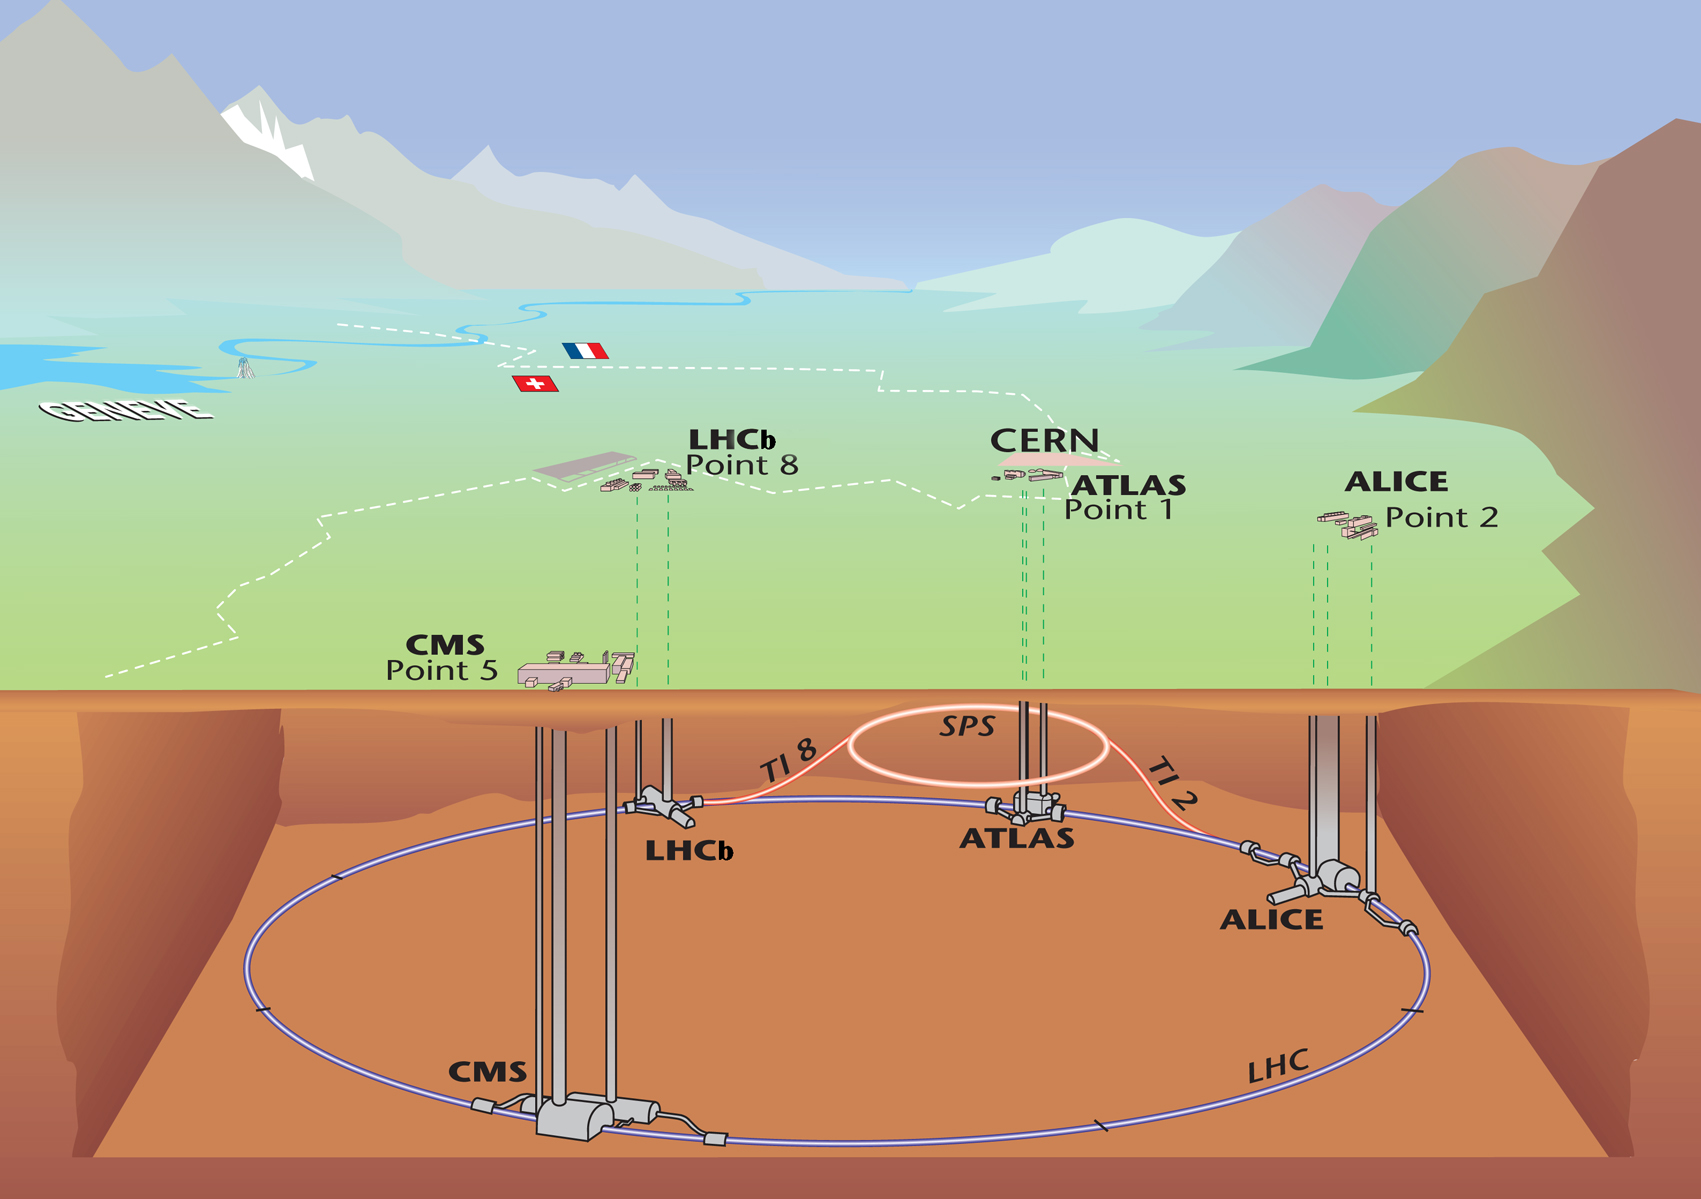
\includegraphics[width=10cm]{CMS_chapter_plots/lhc}
  \caption{Overall view of the LHC experiments \label{fig:LHC}}
\end{figure}
\noindent


\section{CMS Detector}

The central feature of the CMS apparatus is a superconducting solenoid of \unit[6]{m} internal diameter, providing a magnetic field of \unit[3.8]{T}.\\
\indent
Within the superconducting solenoid volume are a silicon pixel and strip tracker, a lead tungstate crystal electromagnetic calorimeter (ECAL), and a brass and scintillator hadron calorimeter (HCAL), each composed of a barrel and two endcap sections. Muons are measured in gas-ionization detectors embedded in the steel flux-return yoke outside the solenoid. Extensive forward calorimetry complements the coverage provided by the barrel and endcap detectors.\\

\begin{figure}[H]
  \centering
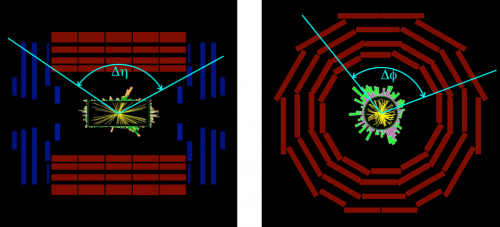
\includegraphics[width=12cm]{CMS_chapter_plots/image_eta}
\label{eta}\caption{$\eta$ and $\phi$ coordinates in the CMS detector}
\end{figure}
\noindent
\indent
A right-handed coordinate system is used with its origin at the nominal interaction point (IP). The x-axis points to the center of
the LHC ring, the y-axis is vertical and points upward, and the z-axis is parallel to the counterclock-wise beam direction. The azimuthal angle $\phi$ is measured with respect to the x-axis in the xy-plane and the polar angle $\theta$ is defined with respect to the z-axis, while the pseudorapidity is defined as $\eta = -\ln\left[\tan\left(\theta/2 \right)  \right]$. 

\begin{figure}[h]
  \centering
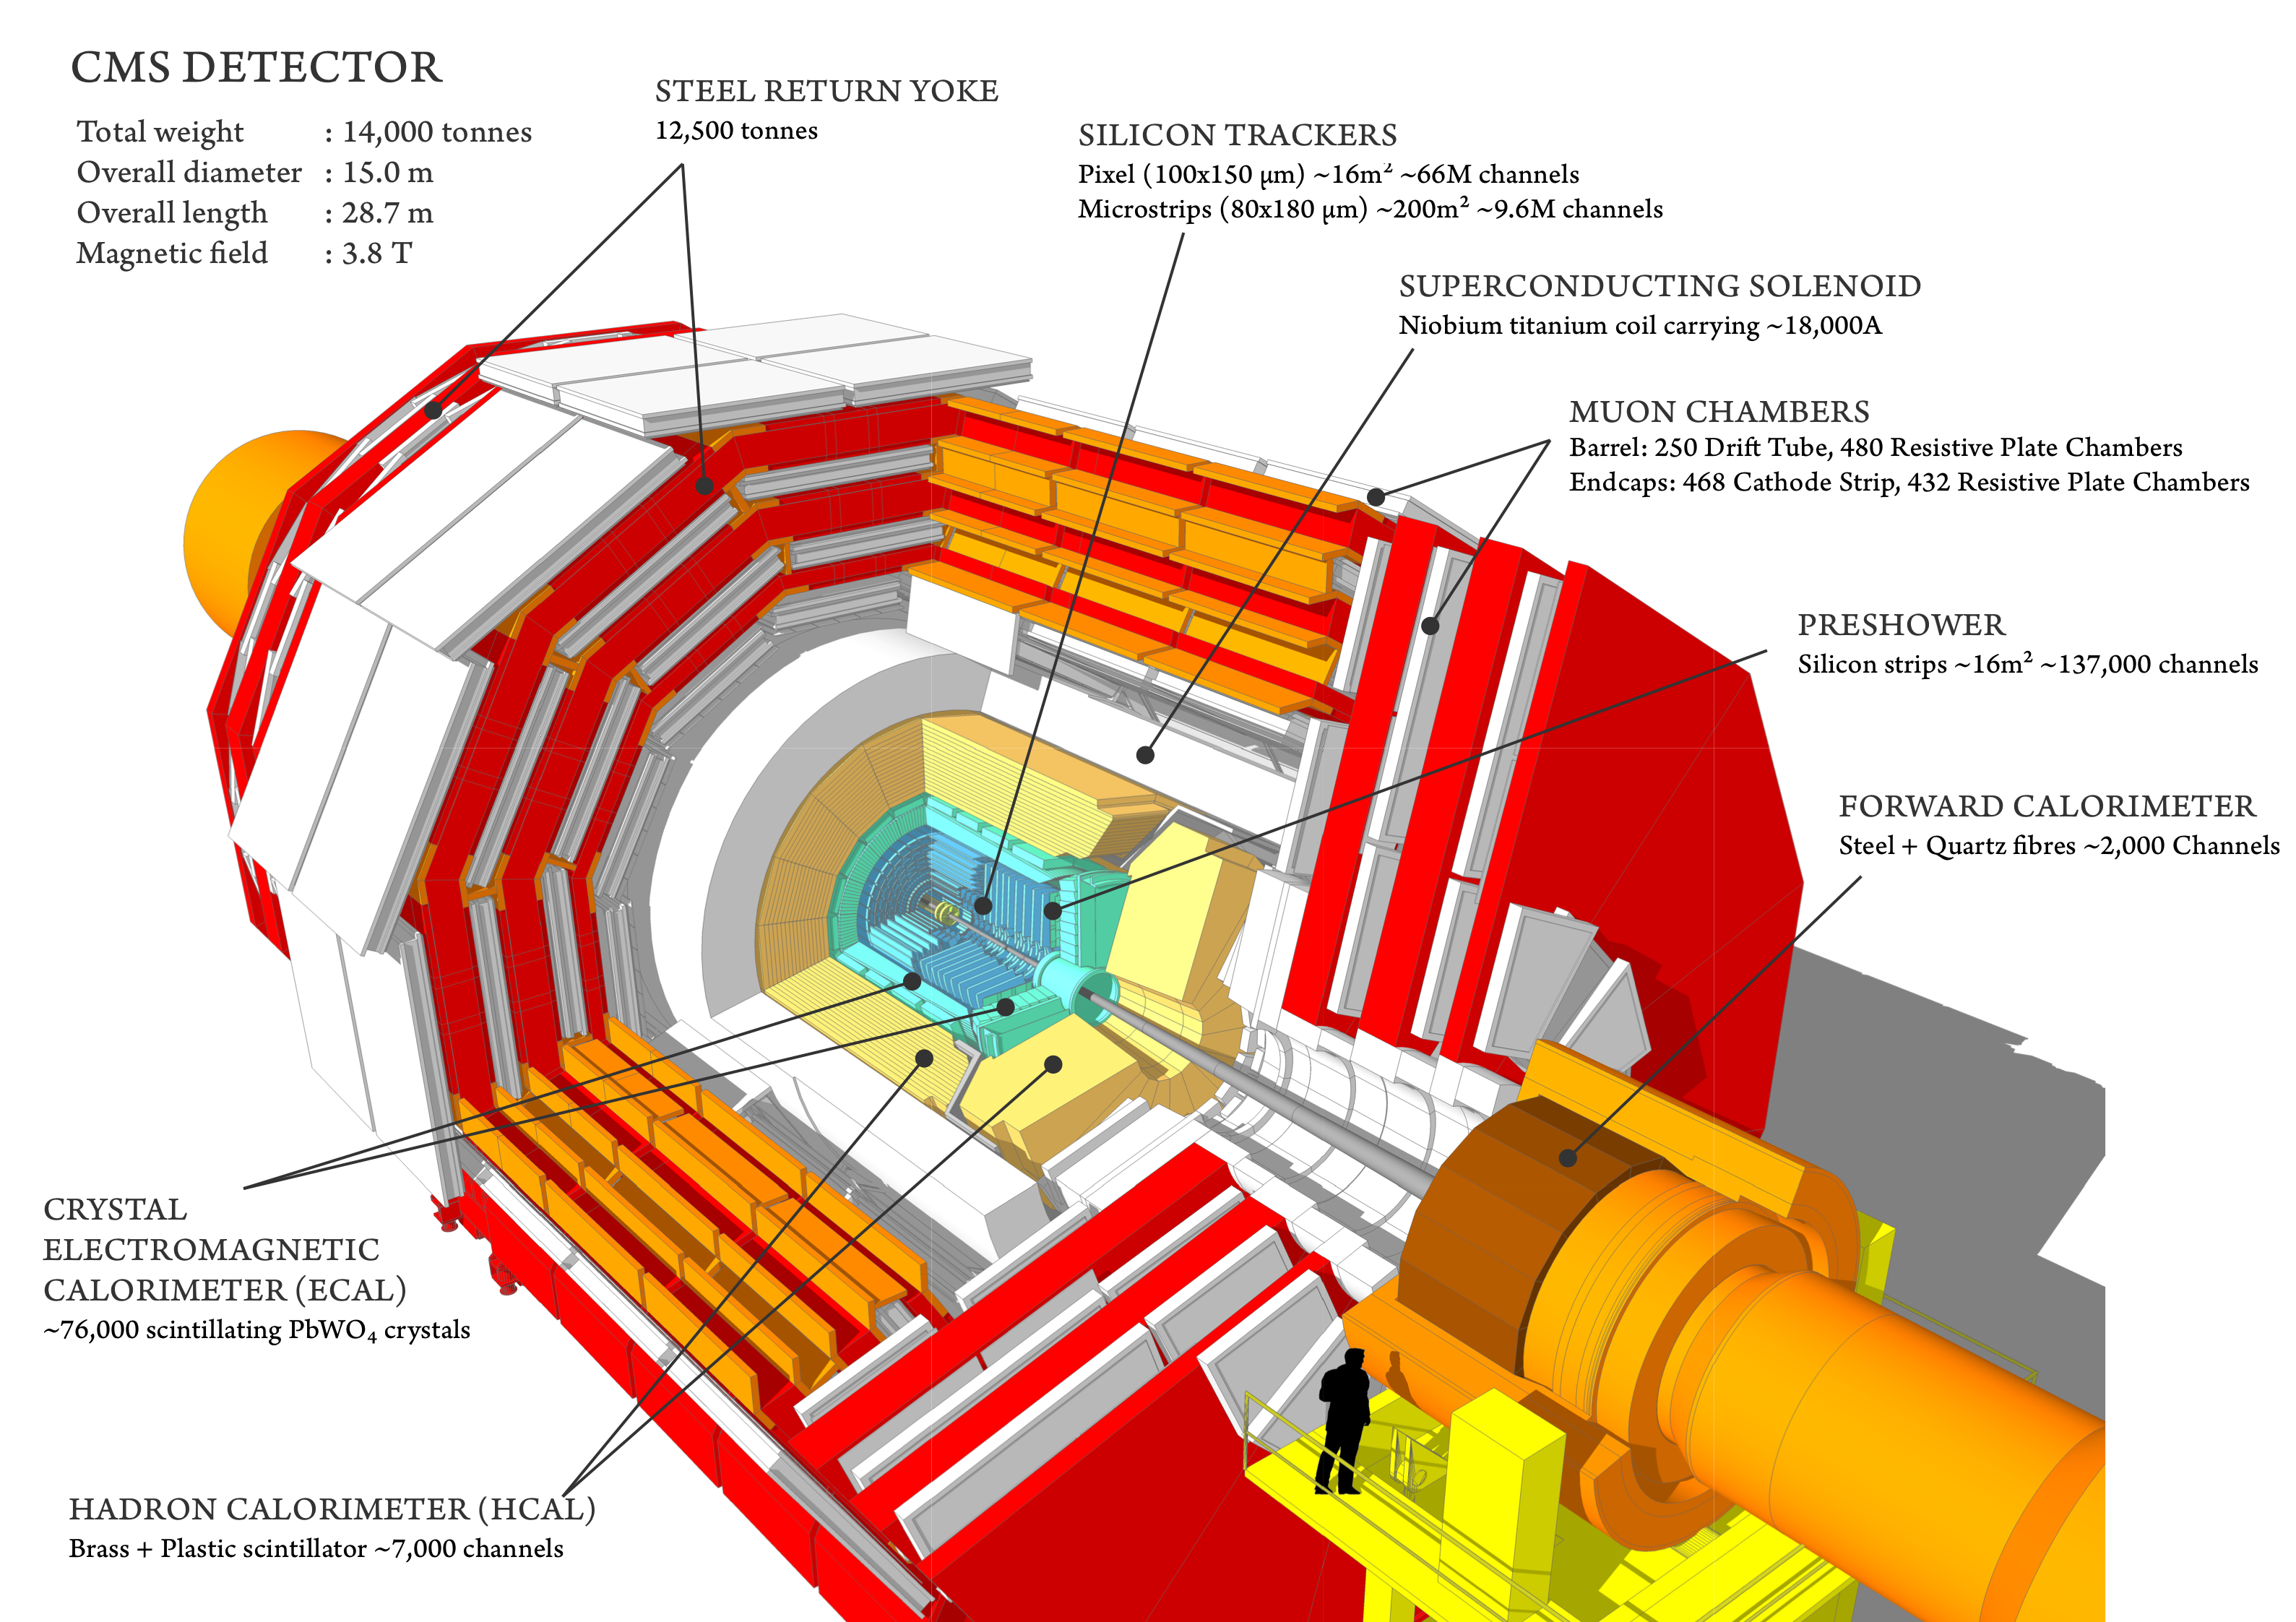
\includegraphics[width=15cm]{CMS_chapter_plots/cms_120918_03}
\label{figure}\caption{Schematic view of the CMS detector}
\end{figure}


\subsection{CMS sub-detectors and components}

\subsubsection{The Magnet}

The CMS collaboration has decided to operate the magnet at a central magnetic flux density
of 3.8 T. After the first years of operation, once the aging of the coil is better understood, the
collaboration may decide to operate the magnet at 4 T.

Since the magnet is the main component of CMS in terms of size, weight and structural
rigidity, it is used as the principal structural element to support all barrel detector components.


Its magnet consists mainly of three parts: a superconducting coil, a vacuum tank and the magnet yoke. The solenoid produces an axial field whereas the yoke is responsible for the return of the magnetic flux. Due to the general design of the CMS detector, the yoke is split into a cylindrical central part, the barrel, and at the extremities, two endcaps made of 600 $\mm$ thick disks.


The yoke contributes to only 8$\%$ of the central magnetic flux density; its main role
is to increase the field homogeneity in the tracker volume and to reduce the stray field by returning
the magnetic flux of the solenoid. In addition, the steel plates play the role of absorber for the four
interleaved layers (“stations”) of muon chambers, which provide for a measurement of the muon
momentum independent of the inner tracking system.




\subsubsection{CMS Tracking system}

The main idea behind "tracking" is to measure the momentum of the particles. The hole tracking system is enclosed in a huge solenoid magnet, which produces an approximately uniform magnetic field pointing along the direction on the LHC beam. As the charged particle flies from the center of the detector, its trajectory are bended. Along its path, it leaves hits in the detecting material.
In a process called track reconstruction, CMS software connects the hits and produces a track. Although we only need three layers to find the particle's paths we actually have many more in order to get a final result for the path that is more accurate.\\
\indent
There will actually be many particles passing through the detector at the same time, so we need lots of measurements to be sure that we are seeing the real track.
If we know the charge of the particle, the intensity of the magnetic field and the radius of the path, we can calculate its transverse momentum.\\
\indent
The tracking system is divide into two different subsystems, the Silicon Pixels and the Silicon Strips.

\paragraph{Silicon Pixels} The CMS pixel detector consists of about 65 million distinct pixels spread over three cylinders of a meter long and in radius of \unit[4]{cm}, \unit[7]{cm} and \unit[10]{cm} (\cref{fig:pixel}).\\
\indent
When a particle passes through our silicon detector, it produce a electron-hole pairs. These electron-hole pairs are pulled in opposite directions by an electric field, and pulled into "contacts". Then, the charge built up on those contacts produces a current that flows into our electronics.\\
\indent 
The key feature of a pixel detector is that the individual contacts are two-dimensional; for every 0.05 by 0.4 millimeter pixel, there is a separate circuit and separate electronics. This gives us a very precise measurement of where, exactly, the particle passed through the detector.
\begin{figure}[H]
  \centering
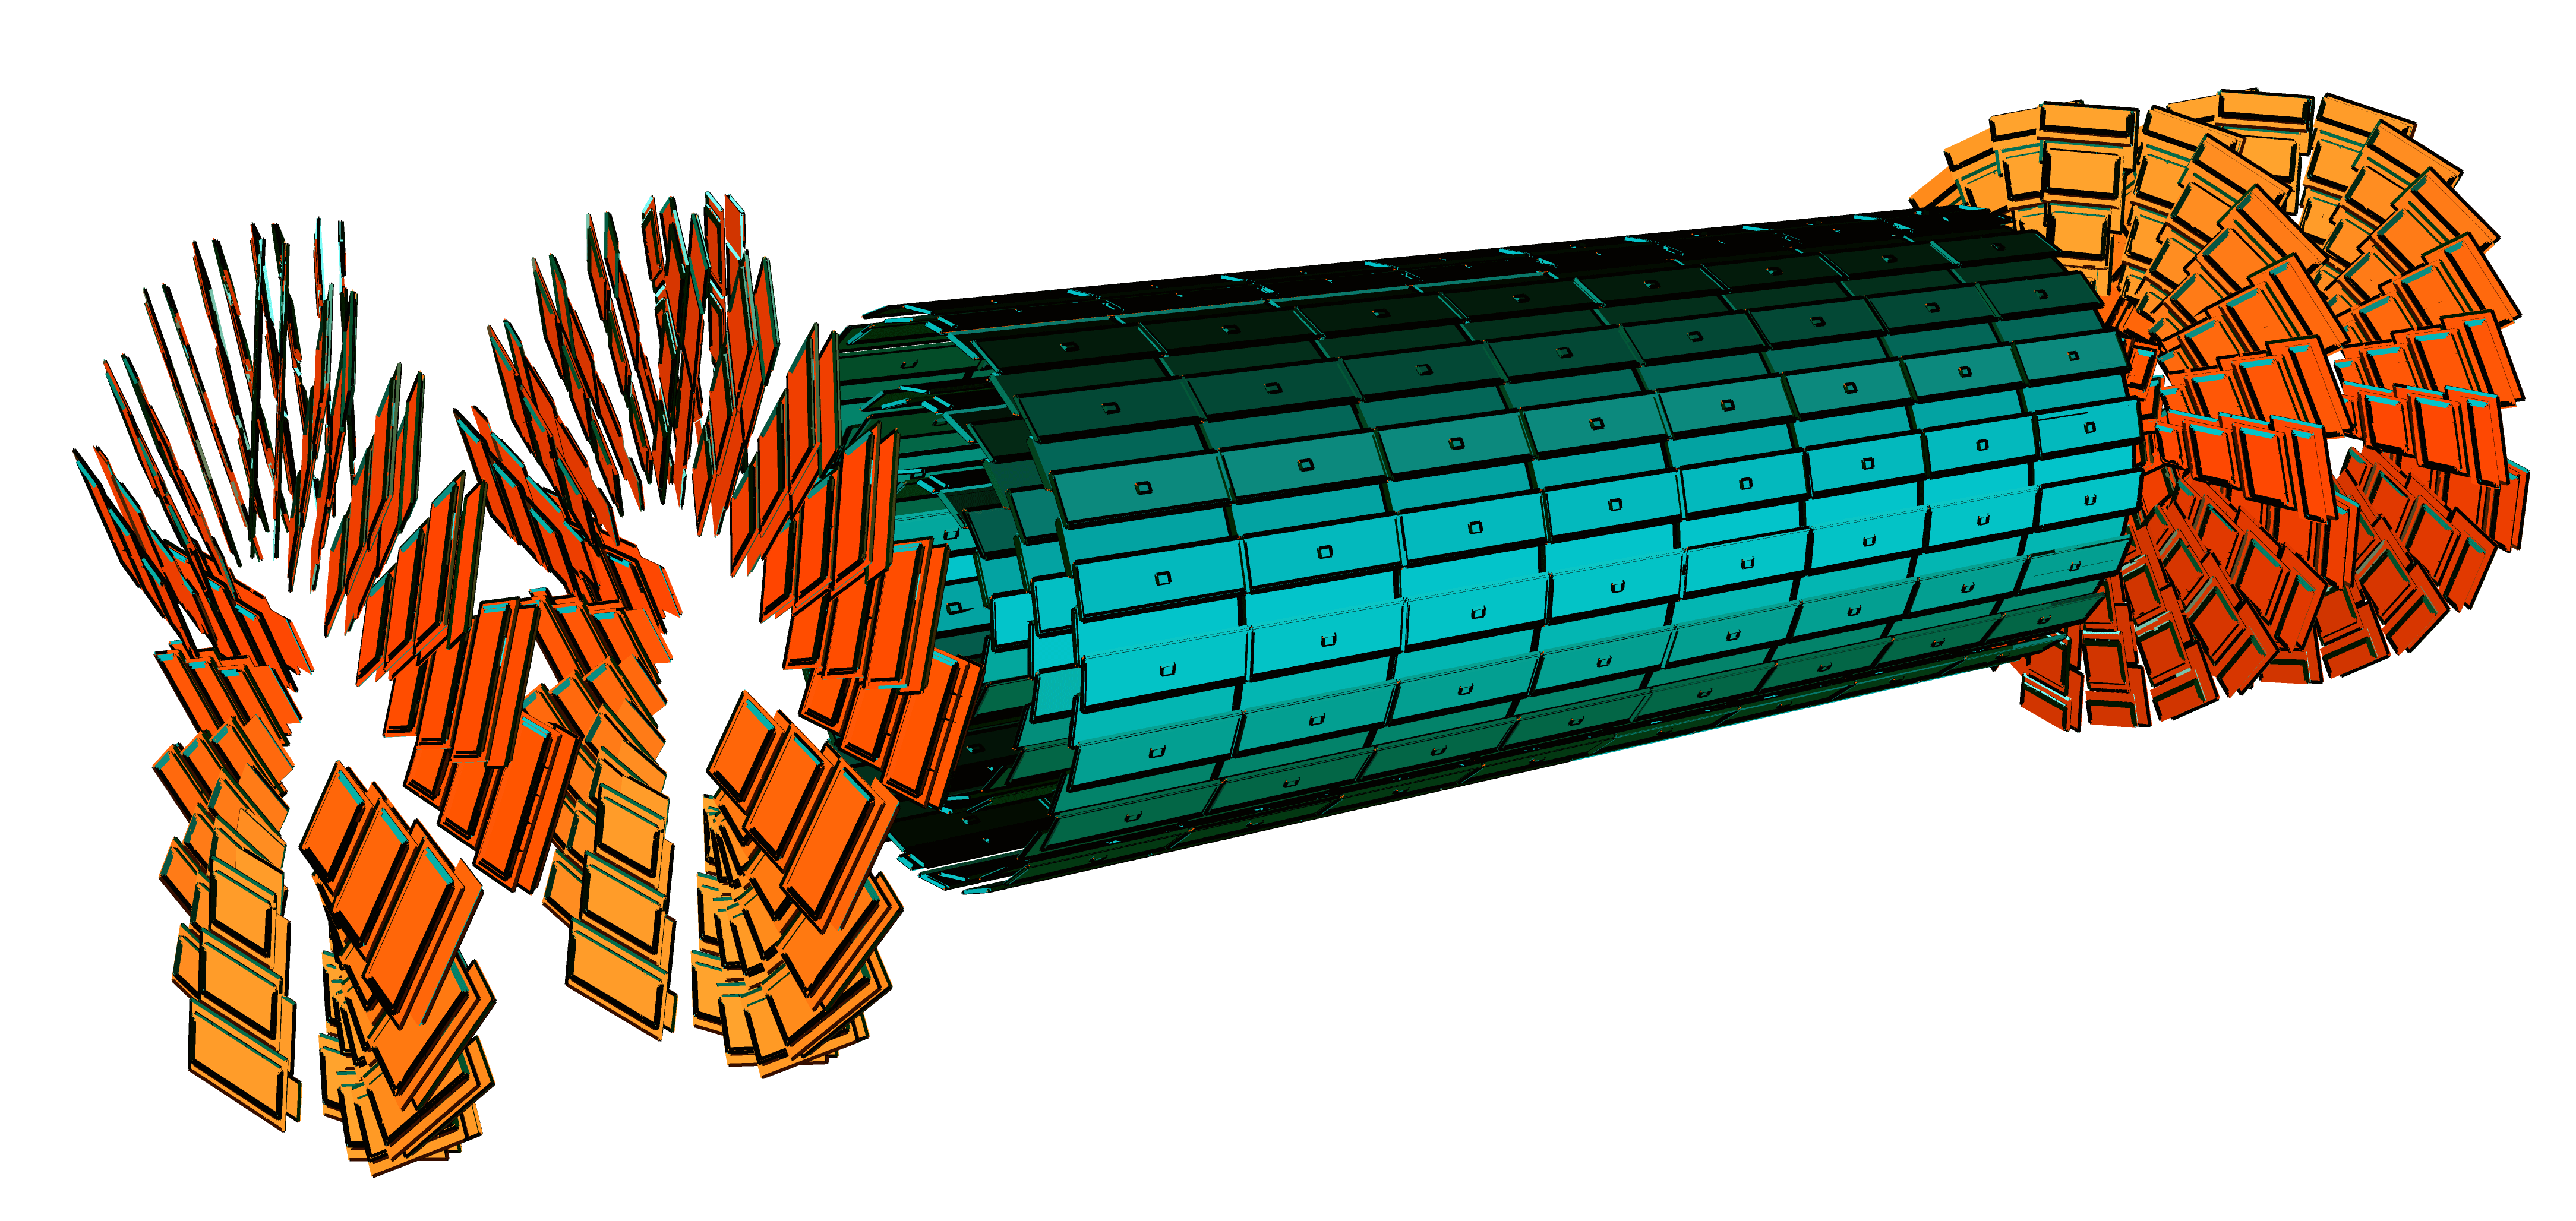
\includegraphics[width=10cm]{CMS_chapter_plots/pixel2}
  \caption{Pixel Detector \label{fig:pixel}}
\end{figure}

\paragraph{Silicon Strips}

The SST consists of four main subsystems, shown in \cref{fig:strip}
: the four-layer Tracker Inner Barrel (TIB), the six-layer Tracker Outer Barrel (TOB) and, on each side of the barrel region, the three-disk Tracker Inner Disks (TID), and the nine-disk Tracker End Caps (TEC).

Each TID disk is made of three rings of modules, while TEC disks have seven rings. The whole SST has a diameter of \unit[2.4]{m} and a length of \unit[5.5]{m}, being the largest silicon detector ever built with an active area of \unit[198]{m$^{2}$}. Its acceptance ranges over a region in pseudo-rapidity $\left| \eta\right|$ < 2.5.

This part of the tracker consist of 15 148 detector
modules and comprises 9.3 million detector channels. Each detector module consists of a carbon or graphite fibre frame, which supports the silicon sensor and the associated front-end readout electronics.
 
The silicon detectors work in much the same way as the pixels: as a charged particle crosses the material it knocks electron from atoms and within the applied electric field these move giving a very small pulse of current lasting a few nanoseconds. This small amount of charge is then amplified by APV25 chips, giving us "hits" when a particle passes, allowing us to reconstruct its path.

The charge on each microstrip is read out and amplified by an Analogue Pipeline Voltage (APV25) chip. Four or six such chips are housed within a “hybrid”, which also contains electronics to monitor key sensor information, such as temperature, and provide timing information in order to match “hits” with collisions. The APV25 stores the signals in a memory for several microseconds and then processes them before sending to a laser to be converted into infrared pulses.


\begin{figure}[H]
  \centering
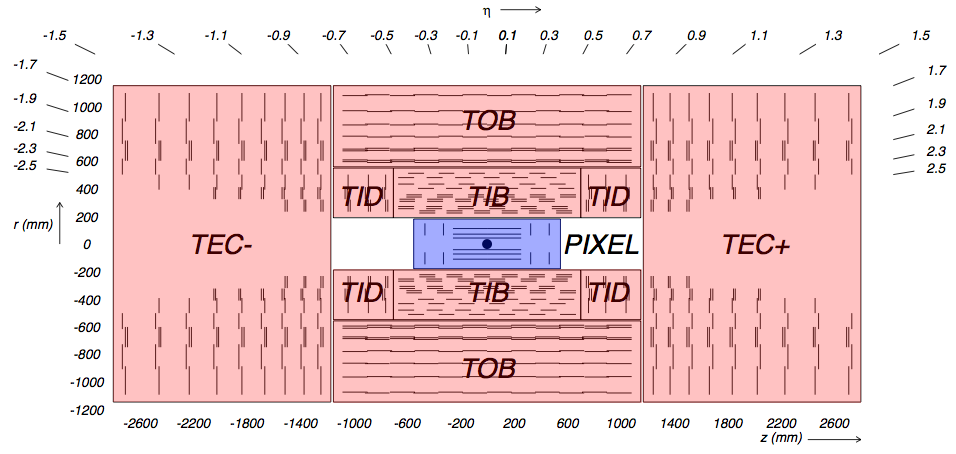
\includegraphics[width=10cm]{CMS_chapter_plots/strip}
  \caption{Strip and Pixel Detector \label{fig:strip}}
\end{figure}

\subsubsection{Electromagnetic Calorimeter (ECAL)}

The ECAL is divided into sections; a barrel section and two endcap sections. The barrel covers the pseudo-rapidity region $\eta$ < 1.48 and is constructed from 61200 lead tungstate crystals. The
crystals are grouped into units, called supermodules, of 1700 crystals. There are 36 supermodules in the barrel.

The endcaps cover the pseudo-rapidity region 1.48 < $\eta$ < 3.0. Each endcap is made from two ‘Dees’ and 7244 crystals. The crystals are grouped into modules of 25 crystals, known as supercrystals. The inner and outer boundaries of the endcaps are made more circular by the addition of smaller units known as partial supercrystals.

\begin{figure}[H]
  \centering
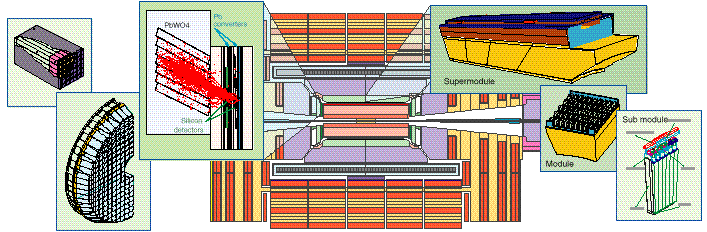
\includegraphics[width=14cm]{CMS_chapter_plots/caloc}
  \caption{Electromagnetic Calorimeter \label{fig:caloc}}
\end{figure}
\noindent
Lead tungstate (PbWO4) is a dense, fast and radiation-tolerant scintillating crystal. These three properties of the crystal make it an ideal choice for the CMS ECAL. The short radiation length and small Moliere radius allow a compact calorimeter to be constructed. The scintillation decay time is very fast with 80$\%$ of the scintillation light collected within 25ns (in the LHC bunches of protons collide every 25ns). 

\subsubsection{Hadronic Calorimeter (HCAL)}

The HCAL \cite{HCAL} is a sampling calorimeter which finds a particle’s position, energy and arrival time using alternating	 layers of "absorber" and fluorescent "scintillator" materials that produce a rapid light pulse when the particle passes through.

Special optic fibres collect up this light and deliver it into readout boxes where photodetectors amplify the signal. When the amount of light in a given region is summed up over many layers of tiles in depth, called a "tower", this total amount of light is a measure of a particle’s energy. 

The hadron calorimeter barrel is radially restricted between the outer extent of the electromagnetic calorimeter (R = 1.77 m) and the inner extent of the magnet coil (R = 2.95 m). This constrains the total amount of material which can be put in to absorb the hadronic shower. Therefore, an outer hadron calorimeter is placed outside the solenoid complementing the barrel calorimeter. Beyond $|\eta| = 3$, the forward hadron calorimeters placed at 11.2 m from the interaction point extend the pseudorapidity coverage down to $|\eta| = 5.2$. 

The HCAL is organized into barrel (formed by two sections : Hadron Barrel(HB) in the region $|\eta|$ < 1.4 and Hadron Outer (HO) in the region $|\eta|$ < 1.26), Hadron Endcap (HE) [1.3<$|\eta|$ < 3.0]  and Hadron Forward (HF) [2.9<$|\eta|$ < 5.0]  sections.(Fig. \ref{fig:hcal1})
\begin{figure}[H]
  \centering
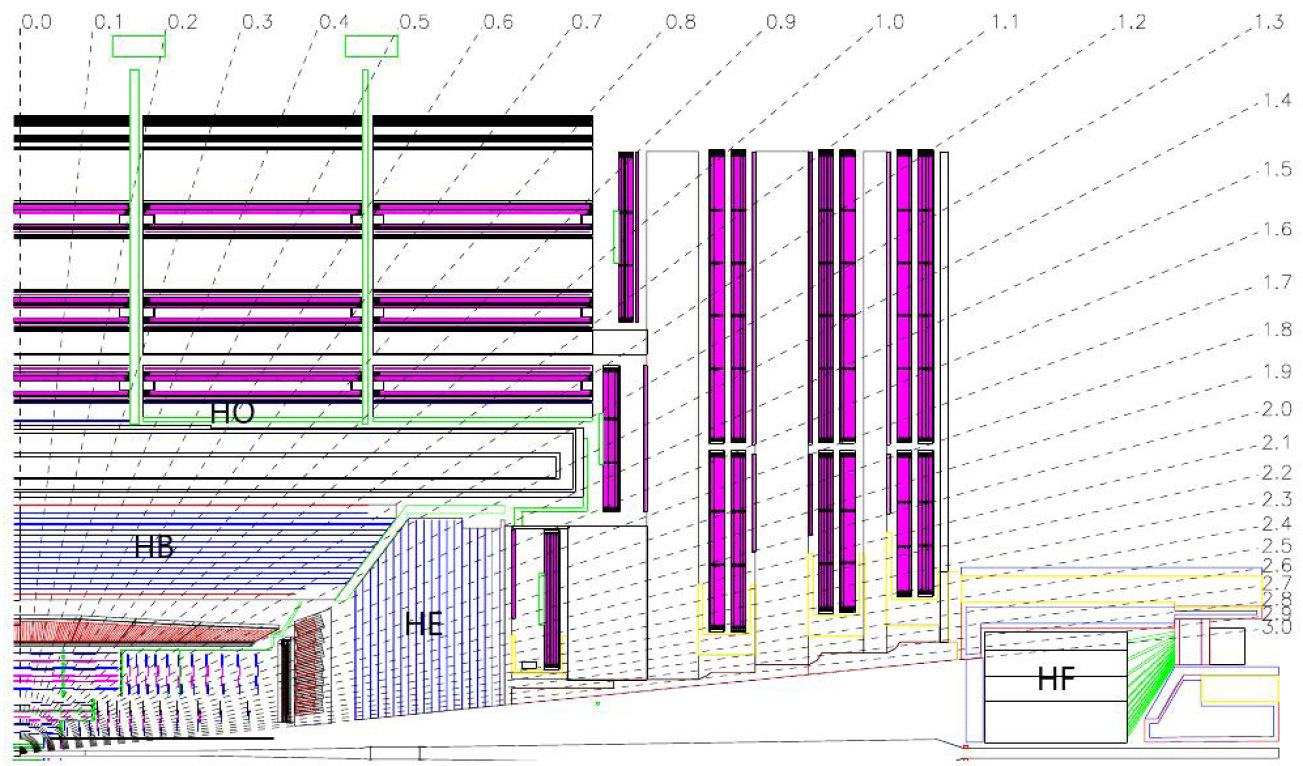
\includegraphics[width=9cm]{CMS_chapter_plots/hcal1}
  \caption{Longitudinal view of the CMS detector showing the locations of the hadron barrel
  (HB), endcap (HE), outer (HO) and forward (HF) calorimeters. \label{fig:hcal1}}
\end{figure}

The HB is a sampling calorimeter covering the pseudorapidity range $|\eta|$ < 1.4, resulting in 2304 towers with a segmentation $\Delta\eta\times\Delta\phi=0.087\times 0.087$.
The HB consists of 36 identical azimuthal wedges which form the two half-barrels (HB$+$ and HB$-$).
\begin{figure}[H]
  \centering
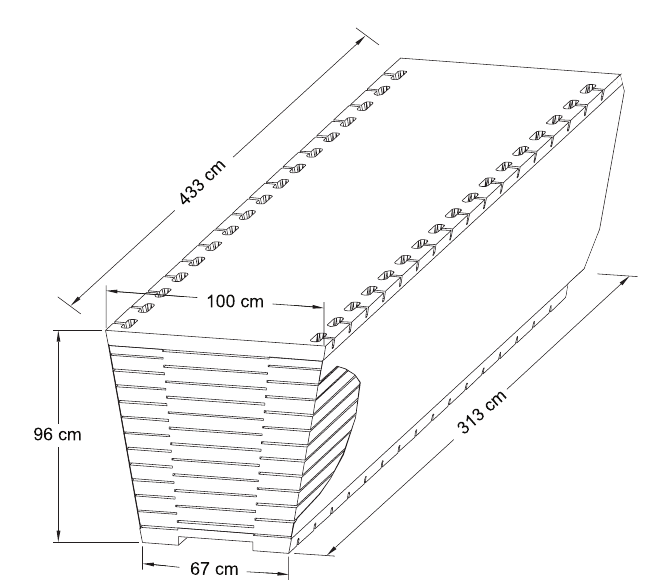
\includegraphics[width=8cm]{CMS_chapter_plots/hcal3}
  \caption{View of an HB wedge. \label{fig:hcal3}}
\end{figure}

The wedges (Fig. \ref{fig:hcal3}) are constructed out of flat brass absorber plates aligned parallel to the beam axis.
The HB baseline active material is 3.7 mm thick Kuraray SCSN81 plastic scintillator, chosen for its long term stability and moderate radiation hardness.

The granularity of the HCAL is 25 times coarser than that of
the ECAL, which would not allow charged and neutral hadrons to be spatially separated in jets with a transverse momentum much above 100 GeV/c. The hadron energy resolution in the combined ECAL-HCAL system is, however, of the order of 10$\%$ at 100 GeV. This resolution allows neutral hadrons to be detected as an energy excess on top of the energy deposited by the charged hadrons pointing to the same calorimeter cells.

More details about the Hadronic Calorimeter may be found in \cite{HCAL2, HCAL3, HCAL4, HCAL5}.

\subsubsection{The Muon System}
\noindent Quality muon detection is one of CMS's most important function. From its earliest conceptual stages, robust and precise muon detection has been the central theme.

Muons can penetrate several metres of iron without interacting. Unlike most particles they are not stopped by any of CMS's calorimeters ($\tau \approx$ 2.2 $\mu$s). Therefore, chambers to detect muons are placed at the very edge of the experiment where they are the only particles likely to register a signal. 

\noindent
The CMS muon system is designed to have the capability of reconstructing the momentum and charge of muons over the the entire kinematic range of the LHC. 

\noindent
The Muon system is a type of tracking detector, and is divided in two main regions: the Barrel ($|\eta|$< 1.2) and  the endcap (1.2 <$|\eta|$< 2.4).\\
There are three types of detectors in the Muon System:

\paragraph{Drift Tubes (DT)}
The drift tube (DT) chamber (Fig. \ref{fig:DT}) system measures muon positions in the barrel part of the detector.

The chamber volume is filled with a Ar(85 $\%$)/CO$_{2}$(15 $\%$) gas mixture, kept at atmospheric pressure.  When a muon or any charged particle passes through the volume, it knocks electrons off the atoms of the gas. By registering where along the wire electrons hit, as well as by calculating the muon's original distance away from the wire, DTs give two coordinates for the muon’s position.
\begin{figure}[H]
  \centering
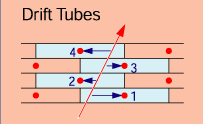
\includegraphics[width=6cm]{CMS_chapter_plots/DT}
  \caption{Muon Drift Tubes \label{fig:DT}}
\end{figure}
\paragraph{Cathode Strip Chamber (CSC)}
Cathode strip chambers (CSC) are used in the endcap disks where the magnetic field is inhomogeneous and particle rates are high.

CSCs consist of arrays of positively charged "anode" wires crossed with negatively charged copper "cathode" strips within a gas volume.

When muons pass through, they knock electrons off the gas atoms, which flock to the anode wires creating an avalanche of electrons. Positive ions move away from the wire and towards the copper cathode, also inducing a charge pulse in the strips, at right angles to the wire direction.
\begin{figure}[H]
  \centering
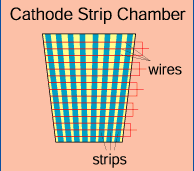
\includegraphics[width=5cm]{CMS_chapter_plots/CSC}
  \caption{Cathode Strip Chamber \label{fig:CSC}}
\end{figure}

\paragraph{Resistive Plate Chambers (RPC)}
Resistive plate chambers (RPC) are fast gaseous detectors that provide a muon trigger system parallel with those of the DTs and CSCs.

RPCs consist of two parallel plates, a positively-charged anode and a negatively-charged cathode, both made of a very high resistivity plastic material and separated by a gas volume.

When a muon passes through the chamber, electrons are knocked out of gas atoms. These electrons in turn hit other atoms causing an avalanche of electrons. The electrodes are transparent to the signal (the electrons), which are instead picked up by external metallic strips after a small but precise time delay. The pattern of hit strips gives a quick measure of the muon momentum, which is then used by the trigger to make immediate decisions about whether the data are worth keeping. 

RPCs combine a good spatial resolution with a time resolution of just one nanosecond (one billionth of a second).
\begin{figure}[H]
  \centering
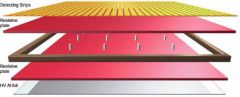
\includegraphics[width=5cm]{CMS_chapter_plots/RPClayers}
  \caption{Resistive Plate Chambers \label{fig:RPClayers}}
\end{figure}


In total there are 1400 muon chambers: 250 drift tubes (DTs) and 540 cathode strip chambers (CSCs) track the particles’ positions and provide a trigger, while 610 resistive plate chambers (RPCs) form a redundant trigger system, which quickly decides to keep the acquired muon data.

The Barrel Detector consists of 4 concentric “stations” (Fig. \ref{fig:mustations}) of 250 chambers inside the magnet return yoke of CMS, which is in turn divided into 5 wheels. Each wheel is divided into 12 sectors, each covering a $30^{\circ}$ azimuthal angle.

The 2 innermost stations, named MS1 and MS2, consist of “sandwiches” made of a DT chamber placed between 2 RPCs. The 2 outermost stations, MS3 and MS4, consist of packages of a DT chamber coupled to a layer made of 1, 2, or 4 RPCs, depending on the sector and station, placed on the innermost side of the station.

\begin{figure}[H]
  \centering
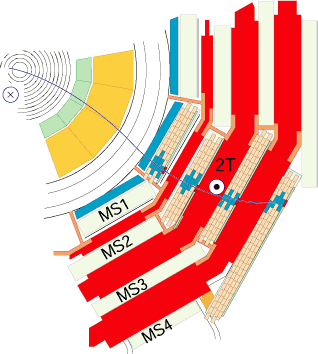
\includegraphics[width=6cm]{CMS_chapter_plots/mustations}
  \caption{Muons Stations \label{fig:mustations}}
\end{figure}

More information about the CMS Muon System may be found in \cite{MUON}.

\subsection{CMS Data Acquisition and Triggering}\label{triggerbase}

When CMS performs at its peak, about one billion proton-proton interactions will take place every second inside the detector. There is no way that data from all these events could be read out, and even if they could, most would be less likely to reveal new phenomena.

We therefore need a "trigger" \cite{TRIGGER1,TRIGGER2} that can select the potentially interesting events, and reduce the rate to just a few hundred "events" per second, which can be read out and stored on computer disk for subsequent analysis.

This task is performed by the trigger system, which is the start of the physics event selection process. The rate is reduced in two steps called Level-1 (L1) Trigger and High-Level Trigger (HLT), respectively. The Level-1 Trigger consists of custom-designed, largely programmable electronics, whereas the HLT is a software
system implemented in a filter farm of about one thousand commercial processors. The rate reduction capability is designed to be at least a factor of $10^{6}$ for the combined L1 Trigger and HLT. 

Level 1 of the trigger is an extremely fast and wholly automatic process that looks for simple signs of interesting physics, e.g. particles with a large amount of energy or in unusual combinations.

The Level 1 trigger select the best 100,000 events each second from the billion available. For the next test, the HLT assimilate and synchronise information from different parts of the detector to recreate the entire event and send it to a farm of more than 1000 standard computers.

\begin{figure}[H]
  \centering
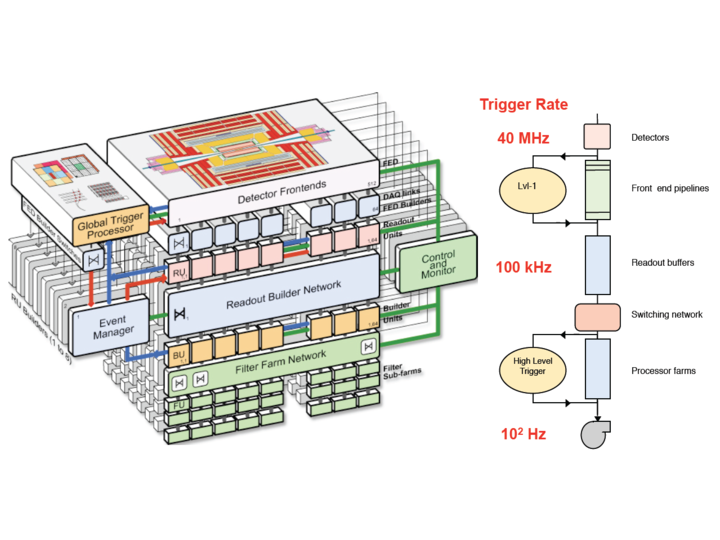
\includegraphics[width=14cm]{CMS_chapter_plots/TRIGGER}
  \caption{CMS Triggering System \label{fig:TRIGGER}}
\end{figure}

Overall they select 100 events per second and the remaining 99,900 are thrown out. We are left with only the collision events that might teach us something new about physics. 

\subsection{Computing and Software}

The CMS Computing Model \cite{COMPUTING} describes how computing centres available to CMS around the world are distributed and configured in a tiered architecture that functions as a single coherent system. It also describes how detector data and MC data travel through the tiers, and how data are distributed, stored, and accessed.

\paragraph{The CMS Data Hierarchy}
CMS Data is arranged into a hierarchy of data tiers. Each physics event is written into each data tier, where the tiers each contain different levels of information about the event. The three main data tiers written in CMS are:
\begin{itemize}
\item 
\textbf{RAW}: full event information from the Tier-0 (i.e. from CERN), containing "raw" detector information (detector element hits, etc)
RAW is not used directly for analysis
        
\item   
\textbf{RECO} ("RECOnstructed data"): the output from first-pass processing by the Tier-0. This layer contains reconstructed physics objects, but it's still very detailed RECO can be used for analysis, but is too big for frequent or heavy use when CMS has collected a substantial data sample.

\item   
\textbf{AOD} ("Analysis Object Data"): this is a condense version of the RECO event information, and is expected to be used for most analyses AOD provides a trade-off between event size and complexity of the available information to optimize flexibility and speed for analyses      
\end{itemize} 

     
\paragraph{CMSSW and Event Data Model (EDM)} 
The overall collection of software, referred to as CMSSW, is built around a Framework, an Event Data Model (EDM), and Services needed by the simulation, calibration and alignment, and reconstruction modules that process event data.

The CMSSW event processing model consists of one executable, called \textit{cmsRun}, and many plug-in modules which are managed by the Framework. All the code needed in the event processing (calibration, reconstruction algorithms, etc.) is contained in the modules. The same executable is used for both detector and Monte Carlo data.

The CMSSW executable, cmsRun, is configured at run time by the user's job-specific configuration file. This file tells cmsRun:

\begin{itemize}
\item 
which data to use
\item 
which modules to execute
\item
which parameter settings to use for each module
\item
what is the order or the executions of modules, called path
\item
how the events are filtered within each path, and
\item
how the paths are connected to the output files 
\end{itemize}

Unlike the previous event processing frameworks, cmsRun is extremely light:only the required modules are dynamically loaded at the beginning of the job.

The CMS Event Data Model (EDM) is centered around the concept of an Event. An Event is a C++ object container for all RAW and reconstructed data related to a particular collision. During processing, data are passed from one module to the next via the Event, and are accessed only through the Event. All objects in the Event may be individually or collectively stored in ROOT files, and are thus directly browsable in ROOT. This allows tests to be run on individual modules in isolation. 


\begin{comment}
\input PhysicsObjects.tex
\input Analysis.tex
\input Conclusions.tex
%\input DataED.tex
%\input Conclusao.tex

%\input cap2.tex
%\input cap3.tex
\appendix
%%% Truque
\renewcommand{\chaptername}%
    {Apêndice}
%\input analise_Zjets.tex
%\input ap1.tex
%\input ap2.tex
%\input ap3.tex
%\bibliography{mibiblio}{}
%\bibliographystyle{unsrtnat}

\begin{thebibliography}{9}

\bibitem{higgsdisco}
CMS Collaboration,
"Observation of a new boson at a mass of 125 GeV with the CMS experiment at the LHC", 
Physics Letters B, Volume 716, Issue 1, 17 September 2012, Pages 30–61.

\bibitem{Randall:1999ee}
Lisa Randall and Raman Sundrum,
"Large Mass Hierarchy from a Small Extra Dimension",
Phys.Rev.Lett. 83.3370 (1999),
\eprint{hep-ph/9905221}.

\bibitem{Randall:1999vf}
Lisa Randall and Raman Sundrum,
An Alternative to Compactification"
Phys. Rev. Lett.83.4690,
\eprint{hep-th/9906064}.

\bibitem{Aga}
Kaustubh Agashe and Hooman Davoudiasl and Gilad Perez and Amarjit Soni,
"Warped Gravitons at the LHC and Beyond",
Phys. Rev. D 76.036006,
\eprint{hep-ph/0701186}.

\bibitem{Fitz}
A. L. Fitzpatrick, J. Kaplan, L. Randall, and L.T. Wang,
"Searching for the Kaluza-Klein Graviton in Bulk RS Models",
JHEP 0709 (2007) 013,
\eprint{hep-ph/0701150}.

\bibitem{HVT}
D. Pappadopulo, A. Thamm, R. Torre, and A. Wulzer, "Heavy Vector Triplets: Bridging Theory and Data", (2014),
\eprint{1402.4431}.

\bibitem{glashow}
S. Glashow,
"Partial-symmetries of weak interactions",
Nucl. Phys. 22 (1961) 579.

\bibitem{weinberg}
S. Weinberg,
"A Model of Leptons",
Phys. Rev. Lett. 19 (1967) 1264.

\bibitem{salam}
A. Salam,
N. Svartholm, ed. Elementary Particle Physics: Relativistic Groups and Analyticity. Eighth Nobel Symposium. Stockholm: Almquvist and Wiksell. p. 367.

\bibitem{higgs}
Peter W. Higgs,
"Spontaneous Symmetry Breakdown without Massless Bosons",
Phys. Rev. 145, 1156  (1966).

\bibitem{goldstone1}
Jeffrey Goldstone, Abdus Salam, and Steven Weinberg,
"Broken Symmetries",
Phys. Rev. 127, 965 (1962).

\bibitem{nambu}
Yoichiro Nambu,
"Axial Vector Current Conservation in Weak Interactions",
Phys. Rev. Lett. 4, 380 (1960).

\bibitem{gold2}
J. Goldstone,
"Field Theories with Superconductor Solutions",
Nuovo Cimento 19: 154–164.

\bibitem{kibble}
T. W. B. Kibble,
"Symmetry Breaking in Non-Abelian Gauge Theories",
Phys. Rev. 155, 1554 (1967).

\bibitem{csaki}
Csaba Csaki,
"TASI Lectures on Extra Dimensions and Branes",
\eprint{hep-ph/0404096v1} (2004)


\bibitem{ArkaniHamed:1998a}
Nima Arkani-Hamed and Savas Dimopoulos and G. R. Dvali
"The Hierarchy problem and new dimensions at a millimeter", 
Phys.Lett. B429 (1998) 263–272, doi:10.1016/S0370-2693(98)00466-3,
arXiv:hep-ph/9803315.

\bibitem{Antoniadis:1998b}
Antoniadis and N. Arkani-Hamed and S. Dimopoulos
\emph{"New dimensions at a millimeter to a Fermi and superstrings at a TeV"}
Phys. Lett.B 436 (1998), arXiv:hep-ph/9804398.

\bibitem{UED}
Thomas Appelquist, Hsin-Chia Cheng, Bogdan A. Dobrescu, 
"Bounds on Universal Extra Dimensions",
Phys.Rev.D64:035002,(2001),
\eprint{hep-ph/0012100}


\bibitem{Goldb}
W. D. Goldberger and M. B. Wise 
\emph{"Phenomenology of a Stabilized Modulus"}
Physics Letters B, Volume 475, Issues 3-4, 2 March 2000, Pages 275-279, arXiv:hep-ph/9911457.

\bibitem{lhc}
Oliver S. Bruning, P. Collier, P. Lebrun, S. Myers, R. Ostojic, J. Poole, P. Proudlock,
"LHC Design Report Vol.1: The LHC Main Ring", CERN-2004-003-V1 (2004).	

\bibitem{HCAL}
  CMS Collaboration,
  \emph{"The Hadron Calorimeter Technical Design Report"},
  CERN/LHCC   97-031 (1997). CMS TDR 2. 
  
\bibitem{HCAL2}  
S. Abdullin et al., \emph{"Design, performance and calibration of the CMS forward calorimeter wedges"}, Eur.Phys.J. C53 (2008) 139–166.

\bibitem{HCAL3}
S. Abdullin et al., \emph{"Design, performance, and calibration of CMS hadron-barrel calorimeter wedges"}, Eur. Phys. J. C55 (2008) 159–171.

\bibitem{HCAL4}
S. Abdullin et al., \emph{"Design, performance, and calibration of the CMS Hadron- outer calorimeter"}, Eur. Phys. J. C57 (2008) 653–663.

\bibitem{HCAL5}
S. Abdullin et al., \emph{"Design, performance, and calibration of CMS hadron endcap calorimeters"}, Europan Journal of Physics C60
(2009) 359–373.

\bibitem{MUON}
  CMS Collaboration,
  \emph{"Muon Technical Design Report"},
  CERN/LHC  97-32 (1997). CMS TDR 3.

\bibitem{TRIGGER1}
  CMS Collaboration,
  \emph{"CMS The TriDAS Project : Technical Design Report, Volume 1: The Trigger Systems"}
   CERN/LHCC-2000-38; CMS TDR 6.1 (2000),  
   \url{https://cds.cern.ch/record/706847/files/cer-002248791.pdf}

\bibitem{TRIGGER2}
  CMS Collaboration,
  \emph{"CMS The TriDAS Project : Technical Design Report, Volume 2: Data Acquisition and High-Level Trigger"}
   CERN-LHCC-2002-026; CMS-TDR-6 (2002), 
   \url{http://cds.cern.ch/record/578006/files/cer-2336481.pdf}
   

\bibitem{COMPUTING}
  CMS Collaboration,
  \emph{"The CMS Computing Model"}, Nuclear Physics B - Proceedings Supplements, Volume 172, October 2007, Pages 53-56.

\bibitem{PF1}  
CMS Collaboration,
\emph{"Particle-Flow Event Reconstruction in CMS and
Performance for Jets, Taus, and MET"}, CMS Physics Analysis Summary
\textbf{PFT-09-001} (2009).

\bibitem{PF2}
CMS Collaboration,
\emph{"Commissioning of the Particle-flow Event
Reconstruction with the first LHC collisions recorded in the CMS detector"},
CMS Physics Analysis Summary
\textbf{PFT-10-001} (2010).

\bibitem{PF3}
CMS Collaboration,
\emph{"Commissioning of the Particle-Flow Reconstruction in
Minimum-Bias and Jet Events from pp Collisions at $\sqrt{s}$ = 7 TeV"},
CMS Physics Analysis Summary
\textbf{PFT-10-002} (2010),
\url{https://cms-physics.web.cern.ch/cms-physics/public/PFT-10-002-pas.pdf}

\bibitem{antikt}
Matteo Cacciari, Gavin P. Salam, Gregory Soyez,
\emph{"The anti-$k_{t}$ jet clustering algorithm"},
JHEP 0804:063, (2008), \eprint{0802.1189}.

\bibitem{fastjet}
Matteo Cacciari, Gavin P. Salam, Gregory Soyez,
\emph{"FastJet user manual"},
The European Physical Journal C 72:1896, arXiv:1111.6097 [hep-ph].  

\bibitem{jetcorrec}
CMS Collaboration,
\emph{"Plans for Jet Energy Corrections at CMS"},
\textbf{CMS PAS JME-07-002}, (2008).

\bibitem{pfjet}
CMS Collaboration,
\emph{"Particle Flow Jet Composition"},
\textbf{CMS AN-2010/005} (2010).    

\bibitem{pileupchs}
CMS Collaboration,
\emph{"Study of Pileup Removal Algorithms for Jets"},
\textbf{CMS PAS JME-14-001} (2014),
\url{https://cds.cern.ch/record/1751454/files/JME-14-001-pas.pdf}

\bibitem{vtagging}
CMS Collaboration,
\emph{"V Tagging Observables and Correlations"},
\textbf{CMS PAS JME-14-002} (2014)

\bibitem{subjetiness}
J. Thaler and K. Van Tilburg,
\emph{"Maximizing Boosted Top Identification by Minimizing
N-subjettiness"},
JHEP 1202 (2012) 093, doi:10.1007/JHEP02(2012)093, arXiv:1108.2701.

\bibitem{softdrop}
A. J. Larkoski, S. Marzani, G. Soyez, and J. Thaler,
\emph{"Soft Drop"},
JHEP 1405 (2014) 146, doi:10.1007/JHEP05(2014)146, arXiv:1402.2657.

\bibitem{pruning}
Stephen D. Ellis, Christopher K. Vermilion, Jonathan R. Walsh
\emph{"Recombination Algorithms and Jet Substructure: Pruning as a Tool for Heavy Particle Searches"},
Phys.Rev.D81:094023,2010, arXiv:0912.0033 [hep-ph].

\bibitem{CaloMET}
CMS Collaboration,
\emph{"Missing $E_{T}$ Performance in CMS"},
CMS Physics Analysis Summary 
\textbf{JME-07-001 (2007)}.

\bibitem{TrackMET}
CMS Collaboration,
\emph{"Track-corrected Missing Transverse Energy in CMS"},
CMS Physics Analysis Summary 
\textbf{JME-09-010 (2009)}.

\bibitem{FiltersMET}
CMS Collaboration,
\emph{"Performance of Missing Transverse Momentum
Reconstruction Algorithms in Proton-Proton Collisions at $\sqrt{s}$ = 8 TeV with the CMS Detector"},
CMS Physics Analysis Summary 
\textbf{CMS-PAS-JME-12-002 } (2012).

\bibitem{TypeIMET}
CMS Collaboration,
\emph{"$\met$ Performance in CMS"},
CMS Analysis Note 
\textbf{CMS AN-2007/041} (2007).

\bibitem{PDG}   
K.A. Olive et al.
\emph{"Particle Data Group"},
Chap 46, KINEMATICS,
Chin. Phys. C, 38, 090001 (2014).

\bibitem{pythia}
T. Sjöstrand, S. Mrenna and P. Skands,
\emph{"A Brief Introduction to PYTHIA 8.1"},
Comput.Phys.Commun. 178, 852-867, (2008) 
\eprint{0710.3820}

\bibitem{madgraph}
J. Alwall, R. Frederix, S. Frixione, V. Hirschi, F. Maltoni, O. Mattelaer, H.-S. Shao, T. Stelzer, P. Torrielli, M. Zaro,
"The automated computation of tree-level and next-to-leading order differential cross sections, and their matching to parton shower simulations",
JHEP07 079 (2014),
\eprint{1405.0301v2}

\bibitem{pat}
W. Adam, V.Adler, B.Hegner, L.Lista, S.Lowette, P.Maksimovic, G. Petrucciani, S.Rappoccio, F.Ronga, R.Tenchini and R.Wolf,
"PAT: The CMS Physics Analysis Toolkit",
J. Phys.: Conf. Ser. 219 032017 doi:10.1088/1742-6596/219/3/032017,
\url{http://iopscience.iop.org/1742-6596/219/3/032017/pdf/1742-6596_219_3_032017.pdf}

\bibitem{jetid}
JME POG (Jet MET Physics Object Group),
\emph{"Jet Identification: Recommendations for 13TeV data analysis"},   
\url{https://twiki.cern.ch/twiki/bin/viewauth/CMS/JetID}   

\bibitem{jetid2}
CMS Collaboration,
\emph{"Performance of the Particle-Flow jet identification criteria
using proton-proton collisions at = 8 TeV"},
\textbf{CMS AN-14-227} (2014)

\bibitem{clean}
CMS Collaboration,
\emph{"PAT Cross Cleaning"},
\url{https://twiki.cern.ch/twiki/bin/view/CMSPublic/SWGuidePATCrossCleaning} 

\bibitem{muonid}
CMS Collaboration,
\emph{"CMS Muon POG"},
\url{https://twiki.cern.ch/twiki/bin/view/CMSPublic/SWGuideMuonId#Loose_Muon.}

\bibitem{muonreco}
CMS Collaboration,
\emph{"Performance of CMS muon reconstruction in pp collision events at $\sqrt{s}$ = 7 TeV"},
JINST 7 P10002 (2012),
\eprint{1206.4071v2}

\bibitem{electronreco}
CMS Collaboration,
"Performance of electron reconstruction and selection with the CMS detector in proton-proton collisions at $\sqrt{s}$= 8 TeV",
JINST 10 P06005 (2015),
\eprint{1502.02701v2}

\bibitem{taureco}
CMS Collaboration,
"Performance of tau-lepton reconstruction and identification in CMS",
JINST 7 P01001 (2012),
\eprint{1109.6034}

\bibitem{HLT}
CMS Collaboration,
\emph{"Instructions for trigger studies"},
\url{https://twiki.cern.ch/twiki/bin/view/CMSPublic/SWGuideTriggerStudiesHowTo}

\bibitem{Trimm} 
David Krohn, Jesse Thaler, and Lian-Tao Wang, 
\emph{"Jet Trimming"},
JHEP 1002:084, (2010), 
\eprint{0912.1342}

\bibitem{Thiagopaper}
CMS Collaboration,
"Search for Randall-Sundrum Gravitons Decaying into
a Jet plus Missing ET at CMS",
CMS Physics Analysis Summary EXO-11-061(2012). \url{http://cdsweb.cern.ch/record/1426654}
 
\bibitem{punzi}
Giovanni Punzi   
\emph{"Sensitivity of searches for new signals and its optimization"},
\eprint{physics/0308063v2}

\bibitem{abcd}
CMS Collaboration,
"Search for Physics Beyond the Standard Model in
Opposite-sign Dilepton Events in pp Collisions at
$\sqrt{s}$ = 7 TeV",
\eprint{1103.1348}

\bibitem{alfametod}
CMS Collaboration,
"Search for new diboson resonances in semileptonic and
hadronic final states at $\sqrt{s}$ = 13 TeV",
CMS AN-15-037 (2015) (Private document)



    
\end{thebibliography}

\end{comment}





\end{document}
